% Local controlled draft for ECOMOD Continued 11, successor to archived Continued 10; 2026-10-28. Not yet an issued release.
\documentclass[11pt,a4paper]{article}
\usepackage[margin=2.4cm]{geometry}
\usepackage{amsmath,amssymb,amsthm}
\usepackage{booktabs,array,tabularx,longtable}
\usepackage{graphicx}
\usepackage{float}
\usepackage[section]{placeins}
\graphicspath{{./}{figures/}}
\usepackage{enumitem}
\usepackage[colorlinks=true,urlcolor=blue,linkcolor=blue,citecolor=blue]{hyperref}
\usepackage[authoryear,round]{natbib}
\emergencystretch=3em
\setlength{\tolerance}{2000}

\renewcommand{\thesection}{S\arabic{section}}
\renewcommand{\theequation}{S\arabic{equation}}
\renewcommand{\thetable}{S\arabic{table}}
\renewcommand{\thefigure}{S\arabic{figure}}
\newtheorem{proposition}{Proposition}
\renewcommand{\theproposition}{S\arabic{proposition}}
\newtheorem{lemma}{Lemma}
\renewcommand{\thelemma}{S\arabic{lemma}}
\newcommand{\pos}[1]{\left[#1\right]_+}
\newcommand{\dconv}{\Delta b_{\mathrm{conv}}}
\newcommand{\Ups}{\Upsilon_c}
\newcommand{\Eceil}{E_{\mathrm{ceil}}}
\newcommand{\Acmin}{A_c^{\min}}
\newcommand{\tconv}{\tau_{\mathrm{conv}}}

\title{Supplementary Information for\\[4pt]
\large Aggregate biocapacity does not identify its composition: a two-land model of ecological-capital drawdown}
\author{Amin Abaee\\ \small Independent Researcher, Tehran, Iran\\ \small amin\_abaee@ut.ac.ir \quad ORCID 0000-0002-0019-1842}

\begin{document}
\maketitle

\noindent Equation numbers without the prefix S refer to the main text.

\section{Symbols and model extensions}\label{si:symbols}

A global hectare (gha) is a hectare normalized to world-average biological productivity for the relevant accounting year. Annual Ecological Footprint and biocapacity account flows are expressed in gha, with the annual basis implicit in the account year \citep{GFNStandards2009,GFNGuidebook2019}. In the model, $B$ and $E$ are annual account-equivalent quantities; in the empirical analysis, $B$ and $E_{\mathrm{prod}}$ are observed NFA account values. The model contributions $Y_f$ and $Y_c$ and shortfall $S$ are expressed in gha, but are not separately reported NFA series. The leaky debt state $D$ is the time-integral of the model shortfall in gha\,yr; $\dot D$ and $\eta D$ are in gha.

\begin{longtable}{>{\raggedright\arraybackslash}p{0.12\textwidth}>{\raggedright\arraybackslash}p{0.41\textwidth}>{\raggedright\arraybackslash}p{0.2\textwidth}>{\raggedright\arraybackslash}p{0.14\textwidth}}
\caption{Symbols, meanings, units and roles. Per-hectare yields on the annual account basis are in gha\,ha$^{-1}$; $b_{G,c}$ is a regeneration-value coefficient in gha\,yr\,ha$^{-1}$; annual account quantities are in gha, with the accounting year implicit; the leaky debt state is in gha\,yr.}\label{tab:si_symbols}\\
\toprule
Symbol & Meaning & Unit & Role \\
\midrule
\endfirsthead
\toprule
Symbol & Meaning & Unit & Role \\
\midrule
\endhead
$A_f$ & fast provisioning land (cropland, intensive) & ha & state \\
$A_c$ & ecological-capital land (forest, soil, wetland, long-rotation systems; effective class) & ha & state \\
$A_r$ & reserve land, $A_{tot}-A_f-A_c$ & ha & dependent balance \\
$q$ & uncalibrated, model-defined capital-land quality index; $q\in K_q=[0,q_{\max}]$ & dimensionless & state \\
$P$ & human population & cap & state \\
$D$ & model leaky-debt state (time-integral of model shortfall) & gha\,yr & state \\
$b_f$ & fast-land account yield per hectare, $(b_{f0}+T_b)e^{-\alpha D}$ & gha\,ha$^{-1}$ & derived \\
$\tilde b_f(t)$ & OWID/FAOSTAT cereal yield, a physical productivity sentinel (not all crops) & tonnes\,ha$^{-1}$ & empirical input \\
$\hat b_f(t)$ & Base-anchored index-scaled proxy yield used only in SI S5 & gha\,ha$^{-1}$ & proxy construction \\
$b_{f0}$ & base fast-land yield per hectare & gha\,ha$^{-1}$ & parameter \\
$b_c$ & capital-land direct yield & gha\,ha$^{-1}$ & parameter \\
$b_{G,c}$ & capital regeneration-value coefficient & gha\,yr\,ha$^{-1}$ & parameter \\
$G_c(q)$ & per-ha regeneration of quality, $\rho_cq(1-q/q_{\max})$ & yr$^{-1}$ & rate function \\
$\Ups(q)$ & per-ha capital value, $b_c+b_{G,c}G_c(q)$ (also written $b_{c,\mathrm{eff}}$) & gha\,ha$^{-1}$ & derived \\
$\dconv$ & composition diagnostic, $b_f-\Ups(q)$ & gha\,ha$^{-1}$ & derived \\
$Y_f,\ Y_c$ & fast and capital yields, $b_fA_f$ and $\Ups A_c$ & gha & derived \\
$B$ & model biocapacity $Y_f+Y_c$; or NFA total under its account convention & gha & aggregate \\
$E_{\mathrm{prod}}$ & NFA Global Ecological Footprint of Production & gha & empirical account \\
$E$ & model-defined footprint demand, $eP$ (or exogenous frozen demand) & gha & aggregate \\
$X,\ C$ & crop-proxy account $X=\hat b_fA_f$ and residual $C=B-X$; neither is physical capital & gha & illustrative accounting split \\
$S$ & shortfall, $\pos{E-\sigma_fY_f-\sigma_cY_c}$ & gha & derived \\
$u_c$ & conversion rate, $\min(S/b_f,\,A_c-\Acmin)/\tconv$ & ha\,yr$^{-1}$ & flow \\
$K$ & carrying capacity, $\max(B/e,K_{\min})$ & cap & algebraic \\
$e$ & per-capita footprint & gha\,cap$^{-1}$ & parameter \\
$r$ & intrinsic population growth rate & yr$^{-1}$ & parameter \\
$\rho_c$ & quality-regeneration scenario rate; not estimated & yr$^{-1}$ & scenario parameter \\
$q_{\max}$ & imposed quality admissibility bound; not an estimated threshold & dimensionless & constraint parameter \\
$\mu$ & cropland maintenance rate (reserve$\to$fast) & yr$^{-1}$ & parameter \\
$\eta_f$ & fast-land retirement rate (fast$\to$reserve) & yr$^{-1}$ & parameter \\
$\tconv$ & conversion time constant & yr & parameter \\
$\alpha$ & degradation rate of $b_f$ per unit debt & gha$^{-1}$\,yr$^{-1}$ & parameter \\
$\eta$ & debt-repayment rate & yr$^{-1}$ & parameter \\
$\tau_g,\ \tau_p$ & regeneration and demographic delay settings & yr & scenario parameters \\
$\sigma_f,\ \sigma_c$ & human-available shares of the two flows & dimensionless & parameter \\
$R_{rc}$ & surplus-gated restoration, $\chi_rA_r\pos{B-E}$ (reserve$\to$capital) & ha\,yr$^{-1}$ & gated flow \\
$\chi_r$ & restoration coefficient & gha$^{-1}$\,yr$^{-1}$ & parameter \\
$T_b$ & technology yield increment, $\omega_{Tb}\Delta b/(1+e^{-\kappa_w(t-t_{wave})})$ & gha\,ha$^{-1}$ & off except in SI S8 \\
$\omega_{Tb}$ & activation flag for the technology wave & dimensionless & $0$ baseline; $1$ in SI S8 \\
$\Delta b$, $\kappa_w$, $t_{wave}$ & amplitude, steepness and center of the wave & gha\,ha$^{-1}$;\newline yr$^{-1}$; yr & active only in SI S8 \\
$\Acmin$, $A_r^{\min}$, $A_f^{\max}$, $K_{\min}$ & capital viability floor, reserve floor, arable ceiling, carrying-capacity floor & ha, ha, ha, cap & typed floors \\
$A_{tot}$ & total bioproductive area & ha & parameter \\
$k$ & $\mu/(\mu+\eta_f)$, fast share of non-capital land at equilibrium & dimensionless & derived \\
$B_{eq}(A_c)$ & frozen-demand balance branch, $b_{f0}kA_{tot}-(b_{f0}k-b_c)A_c$ & gha & derived \\
$\Eceil$ & demand ceiling, $B_{eq}(\Acmin)$ & gha & derived \\
$\lambda_{1,2}$ & deficit-side Jacobian eigenvalues & yr$^{-1}$ & derived \\
$R_B,R_A,\psi_f$ & $E/B$, $E/Y_f$, $Y_f/B$ (so $R_A=R_B/\psi_f$) & dimensionless & diagnostics \\
$\phi_0,w_X,w_C$ & base-year cropland share and log-mean weights & dimensionless & empirical decomposition \\
$s_X,\bar s_X,\bar s_C$ & current and average fast-land shares & dimensionless & empirical decomposition \\
$\mathcal R_c(T)$ & recovery metric, $(A_c(T)-A_c^{\mathrm{deg}})/(A_c^{\mathrm{init}}-A_c^{\mathrm{deg}})$ & dimensionless & derived \\
$R_{fc}$, $\chi$ & fast$\to$capital restoration variant, $\chi A_f\pos{B-E}$ & ha\,yr$^{-1}$; gha$^{-1}$\,yr$^{-1}$ & extension (off) \\
$L_c$, $H_c$ & timber liquidation flow $\pos{H_c-\sigma_cY_c}/b_{G,c}$ and its target & ha\,yr$^{-1}$;\newline gha & extension (off) \\
\bottomrule
\end{longtable}

\paragraph{Model extensions.} Timber liquidation and direct fast-to-capital restoration are not included in the reported simulations. Reservations of the human-available shares are considered as a policy extension in SI~\S S6. The technology wave is inactive in the baseline and gate-sign comparison and is activated only in the matched technology-wave experiment in SI~\S S8.

\paragraph{Conventions.} The positive-part operator is exact, conversion proceeds through the time constant $\tconv$, and land area is conserved among $A_f$, $A_c$, and $A_r$. The uncalibrated quality index $q$ evolves separately from land area, with $K_q=[0,q_{\max}]$ and $q_{\max}=1$ imposed as an admissibility bound. The continuous law is $\dot q=\Pi_{T_{K_q}(q(t))}G_c(q(t-\tau_g))$, with $G_c(x)=\rho_cx(1-x/q_{\max})$; the numerical solver projects the velocity before its Euler update and retains an interval clip as a finite-step safeguard. The parameters $\rho_c$ and $\tau_g$ are scenario settings, not estimates. The maintenance term $\mu A_r$ permits a positive fast-land equilibrium. The reserve floor $A_r^{\min}$ and arable ceiling $A_f^{\max}$ are domain constraints; reported trajectories remain within them, with a minimum reserve of $0.80\,ha$ in the drawdown sweeps. The bounds $A_c\ge\Acmin$, $A_f\ge0$, $q\in K_q$, and $K\ge K_{\min}$ are enforced.

\section{Derivations and proofs}\label{si:proofs}

\subsection{The composition identity with varying debt and quality}\label{si:identity}

Differentiating $B=b_fA_f+\Ups(q)A_c$ with $b_f=(b_{f0}+T_b)e^{-\alpha D}$ and substituting Eqs.~(6)--(7) gives the general identity
\begin{equation}\label{eq:si_identity}
\dot B=\dconv\,u_c+b_f\big(\mu A_r-\eta_fA_f\big)+b_{G,c}G_c'(q)A_c\,\dot q+\Ups R_{rc}-\alpha\dot D\,b_fA_f+\frac{\dot T_b}{b_{f0}+T_b}\,b_fA_f .
\end{equation}
The conversion term has the sign of $\dconv$; the quality term has the sign of $G_c'(q)$ (non-negative for $q\le q_{\max}/2$ and non-positive above it, since $\dot q\ge0$). The debt term is non-positive while debt accrues, the technology term is non-negative while the wave rises, and the restoration term is non-negative. Proposition~1 in the main text assumes $T_b\equiv0$, $R_{rc}\equiv0$, and fixed $D$. In the demonstration parameterization, $D$ evolves and reaches $0.20\,gha\,yr$ before decaying. At the initial state, the conversion contribution is $0.21\,\mathrm{gha\,yr^{-1}}$, compared with $-0.005\,\mathrm{gha\,yr^{-1}}$ from fast-land maintenance and retirement and a debt-term magnitude of approximately $0.004\,\mathrm{gha\,yr^{-1}}$. Conversion therefore dominates the initial rate of change in aggregate biocapacity.

\subsection{The deficit-side affine system and its spectrum}\label{si:affine}

On the deficit side with $q=q_{\max}$, $D$ frozen, $R_{rc}=0$ and $S/b_f<A_c-\Acmin$, Eq.~(5) gives $u_c=(E-b_fA_f-b_cA_c)/(b_f\tconv)$, and with $A_r=A_{tot}-A_f-A_c$ Eqs.~(6)--(7) become
\begin{equation}
\frac{d}{dt}\begin{pmatrix}A_f\\A_c\end{pmatrix}=
\begin{pmatrix}-\tconv^{-1}-\mu-\eta_f & -\mu-\dfrac{b_c}{b_f\tconv}\\[8pt]\tconv^{-1} & \dfrac{b_c}{b_f\tconv}\end{pmatrix}
\begin{pmatrix}A_f\\A_c\end{pmatrix}+
\begin{pmatrix}\dfrac{E}{b_f\tconv}+\mu A_{tot}\\[8pt]-\dfrac{E}{b_f\tconv}\end{pmatrix}.
\end{equation}
Hence $\operatorname{tr}J=-\tconv^{-1}(1-b_c/b_f)-\mu-\eta_f$ and $\det J=(\mu+\eta_f)(k-b_c/b_f)/\tconv$ with $k=\mu/(\mu+\eta_f)$. At the baseline $\operatorname{tr}J=-1.0512\,\mathrm{yr}^{-1}$ and $\det J=0.05353\,\mathrm{yr}^{-2}$, and the eigenvalues are
\begin{equation}
\lambda_{1,2}=\tfrac12\Big(\operatorname{tr}J\pm\sqrt{\operatorname{tr}^2J-4\det J}\Big)=-0.0537\,\mathrm{yr}^{-1},\ -0.9975\,\mathrm{yr}^{-1}.
\end{equation}
Because $J$ contains neither $E$ nor the state, its spectrum is constant along the frozen-demand branch. At $E/\Eceil=0.50,\,0.90,\,0.99,\,0.999$, the slow eigenvalue is $\lambda_1=-0.05366\,\mathrm{yr}^{-1}$. It is independent of $\rho_c$ (with $\lambda_1=-0.0537\,\mathrm{yr}^{-1}$ at $\rho_c=0.04,\,0.08,\,0.16\,\mathrm{yr}^{-1}$), varies modestly with $\tconv$ ($-0.0553,\,-0.0537,\,-0.0505,\,-0.0417\,\mathrm{yr}^{-1}$ at $\tconv=0.5,\,1,\,2,\,5\,\mathrm{yr}$), and varies more with $\mu$ ($-0.0254,\,-0.0537,\,-0.1099\,\mathrm{yr}^{-1}$ at $\mu=0.03,\,0.06,\,0.12\,\mathrm{yr}^{-1}$). The slow eigenvalue remains negative throughout these parameter sweeps. The fixed point of the affine system is $A_c^*(E)$ of Eq.~(18), with $A_f^*=k(A_{tot}-A_c^*)$; for $E>\Eceil$ it lies below $\Acmin$, and the trajectory approaches the face $A_c=\Acmin$ asymptotically, with limiting $u_c=0$ and persistent shortfall $S^*=E-\Eceil$. The balance equality $B_{eq}(A_c)=E$ is only one locus in the switched no-conversion set. Under fixed exogenous demand and $D=0$, any maintenance-balanced allocation with $B_{eq}(A_c)\ge E$ has $S=0$ and $u_c=0$; the strict-surplus allocations are no-conversion states, not equality-balance points. In the full endogenous-population system, a positive stationary population with inactive $K_{\min}$ additionally requires $P=K=B/e$, so $E=B$: the no-conversion equilibria form an equality family with $P$ adjusted as land allocation varies. The deficit-side matrix $J$ above is therefore a one-sided active-shortfall linearization; it does not establish two-sided stability of an isolated equality point. At baseline, two members of the full endogenous-population no-conversion equality family on the branch with inactive $K_{\min}$ are $(A_f^*,A_c^*,A_r^*,P^*)=(0.914\,\mathrm{ha},0.824\,\mathrm{ha},0.762\,\mathrm{ha},1.488\,\mathrm{cap})$ and $(1.091\,\mathrm{ha},0.500\,\mathrm{ha},0.909\,\mathrm{ha},1.731\,\mathrm{cap})$, both with $A_r^*/A_f^*=\eta_f/\mu=0.8333$; the second is a sustainable cropland equilibrium supported by maintenance. The reserve-share mode $A_r/A_f\to\eta_f/\mu$ explains why the strict-inequality interval in the delayed-quality demonstration extends to approximately $149\,\mathrm{yr}$, although most conversion is complete within $25\,\mathrm{yr}$.

In the other branch of the minimum ($S/b_f\ge A_c-\Acmin$), $u_c=(A_c-\Acmin)/\tconv$ and the distance to the floor obeys $\frac{d}{dt}(A_c-\Acmin)=-(A_c-\Acmin)/\tconv$: it decays exponentially and never reaches zero in finite time. The floor is therefore approached asymptotically, and operational floor-proximity thresholds depend on the tolerance used to declare proximity (Section~\ref{si:ladder}).

\subsection{Characteristic structure and the population equation}\label{si:char}

The eigenvalues reported in Section~\ref{si:affine} are only those of the reduced $2\times2$ deficit-side land matrix, under fixed quality $q=q_{\max}$, frozen debt, and active shortfall. They are not the spectrum of the full coupled delay system. We do not report a full-system characteristic-root classification. At $q=q_{\max}$ the tangent-cone projection is one-sided and nonsmooth, so the raw smooth-boundary characteristic equation is not a linearization of the projected law. For the baseline constant history and $\rho_c$, the $\tau_g=20$ and $40$ runs have the explicitly verified saturation path described in the main Methods and Results; no universal ceiling-attractor or delay-robustness claim is made.

On a deficit-active face, the debt equation is $\dot D=E-B-\eta D$. For state order $z=(A_f,A_c,q,P,D)$, with $b_f=(b_{f0}+T_b)e^{-\alpha D}$, its current-state derivative row is
\begin{equation}
\frac{\partial\dot D}{\partial z}=\left(-b_f,\,-\Ups(q),\,-b_{G,c}G_c'(q)A_c,\,e,\,\alpha b_fA_f-\eta\right).
\end{equation}
The final entry includes the feedback through $B$: since $\partial b_f/\partial D=-\alpha b_f$, differentiating $E-B-\eta D$ gives $\alpha b_fA_f-\eta$, not just $-\eta$. The cross-derivatives of $b_f$ with respect to $D$ also enter the land-state rows through the conversion flow. At the audit test state, a finite-difference check gives $-0.0271872877267$, versus the corrected analytic derivative $-0.0271872877250$; the omitted-feedback value would be $-0.05$\,yr$^{-1}$.

For the population equation actually used here,
\begin{equation}
\dot P=rP\left(1-\frac{P}{K(t-\tau_p)}\right),\qquad K=\max(B/e,K_{\min}),
\end{equation}
linearization at a positive equilibrium with $P^*=K^*$ and inactive $K_{\min}$ gives
\begin{equation}
\delta\dot P(t)=-r\,\delta P(t)+r\,\delta K(t-\tau_p)=-r\,\delta P(t)+\frac{r}{e}\,\delta B(t-\tau_p).
\end{equation}
With $K$ fixed, the scalar population perturbation has eigenvalue $-r$, independent of $\tau_p$. In the coupled model, delayed capacity is a forcing generated by the other states, so the delayed-self-feedback criterion $r\tau_p<\pi/2$ for the Hutchinson logistic equation \citep{Hutchinson1948} does not classify this population mode; a full coupled spectrum would require the corresponding active-set characteristic system. We do not claim that the full coupled response is non-oscillatory.

\subsection{Debt fixed points beyond the ceiling}\label{si:debt}

For $E>\Eceil$ the limiting capital state is $A_c=\Acmin$, approached asymptotically, and the persistent shortfall feeds the debt. With $B_{eq}(\Acmin;D)=b_{f0}e^{-\alpha D}k(A_{tot}-\Acmin)+b_c\Acmin$, the debt equation $\dot D=E-B_{eq}(\Acmin;D)-\eta D$ has the fixed point $D^*(E)$ solving $\eta D=E-B_{eq}(\Acmin;D)$; the right-hand side is increasing in $D$, so the fixed point is unique and attracting whenever $\eta>\alpha b_{f0}k(A_{tot}-\Acmin)$ ($0.034\,\mathrm{yr}^{-1}<0.05\,\mathrm{yr}^{-1}$ at the baseline). At the baseline, $D^*=1.186$\,gha\,yr at $E=1.158$\,gha and $D^*=5.375$\,gha\,yr at $E=1.238$\,gha, with $B(D^*)=1.099$ and $0.969$\,gha and persistent shortfalls $S^*=0.059$ and $0.269$\,gha. Under frozen demand the debt therefore saturates; it is unbounded only if the shortfall is.

\subsection{Boundedness asymmetry and the crossover shortfall}\label{si:bounded}

From Eq.~(12), $\ln b_f=\ln(b_{f0}+T_b)-\alpha D$. The first term lies in $[\ln b_{f0},\ \ln(b_{f0}+\Delta b)]$, so the technology channel contributes at most $\ln(1+\Delta b/b_{f0})=\ln(1.85/0.85)=0.778$ to $\ln b_f$ at the baseline. From Eq.~(13), $\dot D\le\bar S-\eta D$ with $\bar S$ the running supremum of the shortfall, so $D(t)\le\max\{D(0),\bar S/\eta\}$ and the degradation channel contributes at least $-\alpha\bar S/\eta$. The two are equal when $\bar S=S^\dagger=(\eta/\alpha)\ln(1+\Delta b/b_{f0})=1.296\,\mathrm{gha}$ at the baseline. The fast-land contribution $Y_f=b_fA_f$ shares this structure; the capital-land contribution $\Ups A_c$ is unaffected by either channel. Under the additive law $b_f=b_{f0}+T_b-\alpha D$, both channels are bounded quantities of the same kind ($\Delta b$ against $\alpha D^*$) and the logarithmic asymmetry disappears, the bound above therefore applies to the multiplicative specification.

\subsection{Macro-ratio identities}\label{si:ratios}

Define $R_B=E/B$, $R_A=E/Y_f$ and the fast-land share $\psi_f=Y_f/B$; then $R_A=R_B/\psi_f$ is an identity. The direct-yield share within the capital-land contribution, $\psi_c=b_cA_c/Y_c$, is a different quantity and $R_A=R_B/\psi_c$ is false. $R_B=1$ is aggregate balance. With baseline shares $\sigma_f=\sigma_c=1$, $R_A>1$ (demand exceeds the fast-land account yield) is necessary but not sufficient for conversion, because the shortfall requires $E>B=Y_f+Y_c$, not merely $E>Y_f$; with reserved flows the threshold changes. The capital-land area declines when $u_c>R_{rc}$, with $u_c$ given by Eq.~(5). Under the baseline shares, active conversion therefore requires $R_B>1$; in the stated reservation extension $\sigma_f,\sigma_c<1$, conversion and declining capital-land area can occur while $R_B\le1$, so aggregate overshoot is not required in that extension. At the regeneration maximum $q^*=q_{\max}/2$ the direct-yield share of capital value is $b_c/(b_c+b_{G,c}\rho_cq_{\max}/4)=0.758$ at the baseline; this is a property of that point, not a structural constant.
\section{Numerical methods and sensitivity analyses}\label{si:numerics}

\paragraph{Numerical method.} The delay equations are integrated by the method of steps with an explicit first-order Euler scheme. At step $k$, the current states are read at $t_{k-1}$; time-dependent and delayed inputs are evaluated at the next grid time $t_k$, with linear interpolation of delayed histories. The quality velocity $G_c(q(t_k-\tau_g))$ is projected onto $T_{K_q}(q(t_{k-1}))$ before the Euler update; the updated quality is then clipped to $K_q=[0,q_{\max}]$ as a finite-step safeguard. The remaining states are advanced using the computed rates, their stated bounds are applied, reserve area is calculated as $A_r=A_{tot}-A_f-A_c$, and the updated $B$ is stored in the delay history. The positive-part operator is exact. For ordinary runs, pre-run histories $q(s)=q_0$ and $B(s)=B_0$ are constant over $[-\max(\tau_g,\tau_p),0)$. In the technology-wave experiment, both runs use the common no-wave prehistory; the active $T_b(0)$ changes current $B(0)$, and subsequent wave-adjusted $B$ values enter the delayed history used for $K(t-\tau_p)$. The demonstration run and bisection thresholds use $\Delta t=0.05$\,yr; drawdown-depth sweeps use $\Delta t=0.1$\,yr, with selected thresholds evaluated at $0.05$\,yr. For $A_{c0}=1.0$\,ha, the $10^{-6}$\,ha floor-proximity threshold changes from $2.955$ to $2.98$\,cap across these step sizes; threshold values are therefore reported as tolerance- and resolution-dependent bands.

\paragraph{Delayed versus current quality in the regeneration term.} The reported model uses the projected delayed law $\dot q=\Pi_{T_{K_q}(q(t))}G_c(q(t-\tau_g))$. A current-quality comparator, using $G_c(q(t))$ with the same imposed interval, is retained only as a sensitivity check. The quality index is uncalibrated, $q_{\max}=1$ is an imposed admissibility bound, and $\rho_c$ and $\tau_g$ are scenario settings; the comparison is not a validation test. In the baseline history $q(s)=0.9$ with $\rho_c=0.08$\,yr$^{-1}$, the projected paths for $\tau_g=20$ and $40$\,yr both reach $q_{\max}$ at $125/9\approx13.8889$\,yr, before either delay elapses. Their equality is a saturation-induced degeneracy, not general delay robustness. The current-quality comparator extends the demonstration window by $1.3$\,yr; the new floor-threshold run changes by at most $0.001$\,cap across the displayed finite set of delays (Table~\ref{tab:si_delay}).

\begin{table}[htbp]
\centering\small
\caption{Sensitivity to evaluating regeneration at current quality rather than using the projected delayed law. The projected delayed model is the specified model; current quality is a comparator only. Demonstration summaries use $\Delta t=0.05$\,yr and $T=400$\,yr; floor-proximity thresholds use $\Delta t=0.1$\,yr and $T=800$\,yr, with $\tau_p=25$\,yr. Biocapacity and contributions are in gha, land areas in ha, $P_0$ in cap, and delays and step intervals in yr.}
\label{tab:si_delay}
\begin{tabularx}{\textwidth}{>{\raggedright\arraybackslash}Xcc}
\toprule
Quantity & current $q(t)$ & projected delayed $q(t-\tau_g)$ \\
\midrule
Demonstration window with $\dot B>0$, $\dot A_c<0$ (yr) & $150.3$ & $149.0$ \\
Mask-end values $B$, $A_c$, $A_f$ & $0.825,\ 0.808,\ 0.923$ & $0.825,\ 0.808,\ 0.923$ \\
Capital contribution $\Ups(q)A_c$ (initial $\to$ mask end, gha) & $0.08364\to0.04038$ & $0.08364\to0.04038$ \\
Fast-land contribution $Y_f$ (initial $\to$ mask end, gha) & $0.51000\to0.78462$ & $0.51000\to0.78462$ \\
$P_0$ floor threshold ($A_{c0}=1.0$\,ha, $\tau_g=5$\,yr, $\Delta t=0.1$\,yr) & $2.955$ & $2.955$ \\
$P_0$ floor threshold ($A_{c0}=1.0$\,ha, $\tau_g=20$\,yr, $\Delta t=0.1$\,yr) & $2.955$ & $2.954$ \\
$P_0$ floor threshold ($A_{c0}=1.0$\,ha, $\tau_g=40$\,yr, $\Delta t=0.1$\,yr) & $2.955$ & $2.954$ \\
\bottomrule
\end{tabularx}
\end{table}

For $\tau_g=20$ and $40$\,yr, the constant history drives $q$ to the cap before the delayed state first enters the solution, so the quality paths are identical; matching thresholds in those two rows are not evidence that delay is generally unimportant. The values in the table were regenerated for this revision from the v45-derived projected solver (thresholds: $T=800$\,yr, $\Delta t=0.1$\,yr). Their agreement at displayed precision with archived C10 values does not identify the historical code-to-output path.

\paragraph{Well-posedness.} For $\rho_c\ge0$, $q_{\max}>0$, and any admissible continuous history $\phi:[-\tau_g,0]\to K_q$, the quality rate $G_c(\phi)$ is nonnegative and Lipschitz on $K_q$. Before the first hit of $q_{\max}$, the method-of-steps delayed equation therefore has a unique solution; at the upper boundary, tangent-cone projection sets the outward velocity to zero, and the state remains there. The lower bound is invariant because the rate is nonnegative. The remaining model right-hand sides are locally Lipschitz on each stated active set; the positive-part and minimum operators are Lipschitz, and the land/debt/population bounds are enforced as described above. We make no smooth linear-stability claim across the quality ceiling or the shortfall switch; the affine spectrum below is a one-sided deficit-branch result.

\section{Extended model results}\label{si:results}

\subsection{Fast-land yield sweep and parameter sensitivity of the composition diagnostic}\label{si:sweep}

Table~\ref{tab:si_sweep} extends the fast-land yield sweep in Table~2(a) in the main text with the slope of the balance branch. The sign of $\dconv$ remains positive as $b_{G,c}$ varies threefold: at $b_f=0.85$\,gha\,ha$^{-1}$, $\Ups(q^*)=0.058,\,0.066,\,0.074$\,gha\,ha$^{-1}$ for $b_{G,c}=0.4,\,0.8,\,1.2$\,gha\,yr\,ha$^{-1}$, so $\dconv=+0.792,\,+0.784,\,+0.776$\,gha\,ha$^{-1}$.

\begin{table}[htbp]
\centering\small
\caption{Fast-land yield sweep at the baseline (all other parameters fixed): composition diagnostic at $q^*$, eigenvalues of the deficit-side matrix, slope of the balance branch and demand ceiling.}
\label{tab:si_sweep}
\begin{tabular}{l r r r r r}
\toprule
$b_f$ (gha\,ha$^{-1}$) & $\dconv(q^*)$ (gha\,ha$^{-1}$) & $\lambda_1$ (yr$^{-1}$) & $\lambda_2$ (yr$^{-1}$) & $b_fk-b_c$ (gha\,ha$^{-1}$) & $\Eceil$ (gha) \\
\midrule
$0.60$ & $+0.534$ & $-0.0522$ & $-0.975$ & $0.277$ & $0.804$ \\
$0.85$ & $+0.784$ & $-0.0537$ & $-0.998$ & $0.414$ & $1.138$ \\
$1.20$ & $+1.134$ & $-0.0547$ & $-1.014$ & $0.605$ & $1.606$ \\
$2.00$ & $+1.934$ & $-0.0556$ & $-1.029$ & $1.041$ & $2.675$ \\
\bottomrule
\end{tabular}
\end{table}

\subsection{Drawdown-depth ladder}\label{si:ladder}

Table~\ref{tab:si_drawdown} gives the minimum capital land reached during endogenous-demand runs ($A_{f0}=0.6$, $q_0=0.9$, $\tau_g=20$, $\tau_p=25$\,yr, $\chi_r=0.10$, $\Delta t=0.1$\,yr, $T=400$\,yr) on a grid of initial population $P_0$; the full grid (step $0.1$) is in \texttt{si\_drawdown\_depth.csv}. The minimum is reached when the shortfall first closes ($B\ge E$), between $3$ and $25$\,yr after the start depending on $P_0$. At $A_{c0}=1.00$\,ha, the $\tau_g=20$ and $40$\,yr runs have identical quality paths because the baseline history reaches the imposed ceiling before either delay elapses; their matching threshold is saturation-induced degeneracy. The $\tau_g=5$\,yr case is distinct. The finite delay comparison does not establish general delay robustness (SI Table~\ref{tab:si_delay} in \S~\ref{si:numerics}). The depth is continuous and monotone in $P_0$ and in $A_{c0}$. The initial population $P_0$ (cap) at which the minimum comes within $10^{-2}$, $10^{-3}$ and $10^{-4}$\,ha of the floor is $1.8,\,1.9,\,2.1$ ($A_{c0}=0.40$\,ha); $2.2,\,2.3,\,2.4$ ($A_{c0}=0.70$\,ha); $2.6,\,2.7,\,2.8$ ($A_{c0}=1.00$\,ha); $2.8,\,2.9,\,3.0$ ($A_{c0}=1.18$\,ha); the bisection with a $10^{-6}$\,ha floor-proximity tolerance ($\Delta t=0.05$\,yr, $T=1000$\,yr) gives $2.41,\,2.70,\,2.98,\,3.14$\,cap. \par\pagebreak

The thresholds are identical to three decimals for $\chi_r=0.10$ and $\chi_r=0$ ($2.387$ and $2.955$\,cap at $A_{c0}=0.40$ and $1.00$\,ha, $\Delta t=0.1$\,yr).

\begin{table}[htbp]
\centering\small
\caption{Minimum capital land $\min_tA_c$ (ha) reached during the run, by initial capital $A_{c0}$ (rows, ha) and initial population $P_0$ (columns, cap); typed floor $\Acmin=0.05$\,ha.}
\label{tab:si_drawdown}
\begin{tabular}{lrrrrrrrr}
\toprule
$A_{c0}$ $\backslash$ $P_0$ & 1.0 & 1.5 & 2.0 & 2.5 & 2.8 & 3.0 & 3.5 & 4.0 \\
\midrule
$0.4$ & 0.396 & 0.147 & 0.050 & 0.050 & 0.050 & 0.050 & 0.050 & 0.050 \\
$0.7$ & 0.700 & 0.442 & 0.121 & 0.050 & 0.050 & 0.050 & 0.050 & 0.050 \\
$1.0$ & 1.000 & 0.731 & 0.398 & 0.075 & 0.050 & 0.050 & 0.050 & 0.050 \\
$1.18$ & 1.180 & 0.898 & 0.557 & 0.230 & 0.055 & 0.050 & 0.050 & 0.050 \\
\bottomrule
\end{tabular}
\end{table}

\subsection{Recovery metric and the role of the restoration flow}\label{si:recovery}

The recovery metric is $\mathcal R_c(T)=(A_c(T)-A_c^{\mathrm{deg}})/(A_c^{\mathrm{init}}-A_c^{\mathrm{deg}})$, with $\mathcal R_c=0$ no recovery, $1$ full recovery to the reference, $<0$ continued decline and $>1$ over-restoration. Table~\ref{tab:si_recovery} evaluates it on the projected delayed-quality drawdown runs with $A_{c0}=1.0$\,ha ($A_c^{\mathrm{init}}=1.0$\,ha, $A_c^{\mathrm{deg}}=\min_tA_c$ in ha, $T=400$\,yr). Without restoration the capital-land area remains at its minimum because no return flow exists. With the surplus-gated flow, recovery is partial across these six initial-population cases ($\mathcal R_c=0.21$--$0.89$); none reaches the reference. The distinct gate-sign experiment in SI~\S S4 tests other initial states and intervention settings, including cases of over-restoration.

\begin{table}[htbp]
\centering\small
\caption{Recovery of the capital-land area after a demand-driven drawdown ($A_{c0}=1.0$\,ha, $A_{f0}=0.6$\,ha, $q_0=0.9$, $T=400$\,yr): initial population $P_0$ is in cap, initial footprint $E_0$ in gha, capital-land values in ha, and the recovery metric is dimensionless.}
\label{tab:si_recovery}
\begin{tabular}{l r r r r r r}
\toprule
$P_0$ & $E_0$ & $\min_tA_c$ & $t(\min)$ (yr) & $A_c(T)$, $\chi_r=0$ & $A_c(T)$, $\chi_r=0.10$ & $\mathcal R_c(T)$, $\chi_r=0.10$ \\
\midrule
$1.5$ & $0.825$ & $0.731$ & $3.0$ & $0.731$ & $0.969$ & $0.89$ \\
$2.0$ & $1.100$ & $0.398$ & $3.8$ & $0.398$ & $0.677$ & $0.46$ \\
$2.5$ & $1.375$ & $0.075$ & $4.1$ & $0.075$ & $0.433$ & $0.39$ \\
$3.0$ & $1.650$ & $0.050$ & $13.8$ & $0.050$ & $0.328$ & $0.29$ \\
$3.5$ & $1.925$ & $0.050$ & $20.6$ & $0.050$ & $0.278$ & $0.24$ \\
$4.0$ & $2.200$ & $0.050$ & $26.6$ & $0.050$ & $0.250$ & $0.21$ \\
\bottomrule
\end{tabular}
\end{table}

\subsection{Gate-sign phase dependence}\label{si:gates}

The gate-sign comparison begins from a post-drawdown state ($A_c=0.058$\,ha near the floor, $A_f=0.6$\,ha, $q=0.9$, and $P=1.2$\,cap). At a degraded equilibrium with $R_B=1$, $B=E$, so neither the surplus-gated nor deficit-gated restoration flow is active. The reference equilibrium has $A_c^{\mathrm{init}}=0.8225$\,ha and $P^{\mathrm{init}}=1.489$\,cap; the degraded value is $A_c^{\mathrm{deg}}=0.0513$\,ha. All rows use $T_b=0$ and the stated initial state.

\begin{table}[H]
\centering\scriptsize
\setlength{\tabcolsep}{2pt}
\caption{Restoration gate and recovery outcomes at $T=100$ and $900$\,yr. The table reports end-state land areas, population relative to the reference, trajectory extrema, and peak debt $D$ (gha\,yr). Annual account values $B=E$ are in gha; land areas are in ha; population ratios and recovery metrics are dimensionless. Each row approaches $R_B=1$ ($E=B$).}
\label{tab:si_gates}
\begin{tabular}{l r r r r r r r r r r}
\toprule
Policy / gate & $\mathcal R_c(100)$ & $\mathcal R_c(900)$ & $A_c$ & $A_f$ & $A_r$ & $B=E$ & $P/P^{\mathrm{init}}$ & $\min A_r$ & $\max A_c$ & $D_{peak}$ \\
\midrule
none ($R_{rc}=0$) & $-0.00$ & $-0.00$ & $0.051$ & $1.336$ & $1.113$ & $1.138$ & $1.39$ & $1.113$ & $0.057$ & $0.152$ \\
surplus-gated, $\chi_r=0.02$ & $0.69$ & $0.73$ & $0.612$ & $1.030$ & $0.858$ & $0.906$ & $1.11$ & $0.858$ & $0.612$ & $0.152$ \\
surplus-gated, $\chi_r=0.05$ & $1.08$ & $1.07$ & $0.875$ & $0.886$ & $0.738$ & $0.797$ & $0.97$ & $0.724$ & $0.885$ & $0.152$ \\
surplus-gated, $\chi_r=0.10$ & $1.28$ & $1.27$ & $1.030$ & $0.802$ & $0.668$ & $0.733$ & $0.90$ & $0.602$ & $1.092$ & $0.152$ \\
surplus, $\chi_r=0.10$, target cap $A_c^*=0.8225$ & $1.00$ & $1.00$ & $0.822$ & $0.915$ & $0.763$ & $0.819$ & $1.00$ & $0.664$ & $0.822$ & $0.152$ \\
surplus, $\chi_r=0.10$, conversion frozen & $1.35$ & $1.36$ & $1.097$ & $0.765$ & $0.638$ & $0.705$ & $0.86$ & $0.602$ & $1.097$ & $0.543$ \\
deficit-gated, $\chi_r=0.05$ & $0.00$ & $0.00$ & $0.055$ & $1.334$ & $1.112$ & $1.136$ & $1.39$ & $1.112$ & $0.060$ & $0.145$ \\
deficit-gated, $\chi_r=0.10$ & $0.01$ & $0.01$ & $0.059$ & $1.331$ & $1.110$ & $1.135$ & $1.39$ & $1.110$ & $0.065$ & $0.139$ \\
deficit, $\chi_r=0.10$, conversion frozen & $0.05$ & $0.05$ & $0.088$ & $1.315$ & $1.096$ & $1.123$ & $1.37$ & $1.096$ & $0.088$ & $0.159$ \\
\bottomrule
\end{tabular}
\end{table}

Without restoration, $A_c$ remains at its minimum because the model has no return flow. Surplus-gated restoration yields partial or over-restoration depending on $\chi_r$; at $\chi_r\ge0.05$, the flow continues while $B>E$, and the supported population falls to $0.97$--$0.90$ of its reference value. A target cap returns $A_c$ to its reference value ($\mathcal R_c=1.00$). Deficit-gated restoration acts during the shortfall, but at the tested rates its contribution is smaller than concurrent conversion and the recovery fraction remains near zero. Freezing conversion under surplus-gated restoration raises peak debt from $0.152$ to $0.543$\,gha\,yr; restoration then reallocates reserve area to capital land while fast-land maintenance is reduced. These outcomes depend on the specified initial state and intervention rates. The gate-sign comparisons use $T_b=0$; the controlled wave/no-wave debt comparison is reported in SI~\S S8.\par\pagebreak

\subsection{Regime table}\label{si:regimes}

\begin{table}[H]
\centering\small
\caption{The composition diagnostic $\dconv$ (gha\,ha$^{-1}$) as the decision condition for mask visibility. There is no interior area-based capacity maximum in the quality-based model; the only shape distinction is the sign of $\dconv$.}
\label{tab:si_regime}
\begin{tabularx}{\textwidth}{l l X}
\toprule
Regime & Condition & Behavior \\
\midrule
composition-premium & $\dconv>0$ & the conversion contribution to accounting $B$ is positive; net $B$ also depends on other flows (the mask is possible in the baseline) \\
composition-neutrality & $\dconv=0$ & first-order neutrality; non-generic \\
composition-discount & $\dconv<0$ & conversion lowers $B$ at the conversion margin; conversion alone cannot produce a composition mask \\
\bottomrule
\end{tabularx}
\end{table}

\section{Empirical details}\label{si:empirical}

\subsection{Data and vintages}\label{si:vintages}

The empirical backbone is the National Ecological Footprint and Biocapacity Accounts (NFA), Edition 2026, results and metadata version 1.0 \citep{Lo2026NFA}. Although the workbook covers 1961--2025, the primary analysis uses complete world observations for 1961--2023; the 2024--2025 estimated rows are excluded. The 1961--2022 sensitivity uses the same edition and population series. The release recalculates common historical years and reports biocapacity by fishing grounds, built-up land, cropland, grazing land, and forest biocapacity. These are account categories, not a common-boundary physical-stock inventory.

The workbook's $\texttt{pop\_1000\_persons}$ field is UN PopStat population in thousands of persons; it is converted to persons before recomputing per-capita values. The field $\texttt{efp\_total\_gha}$ is the Global Ecological Footprint of Production, denoted $E_{\mathrm{prod}}$ here. Per-capita values are ratios of the unrounded account totals and population, not the workbook's rounded per-capita columns. Table~\ref{tab:si_nfa_endpoints} summarizes endpoint changes. For 1961--2023, $B$ is $9{,}725{,}417{,}562$ to $12{,}142{,}843{,}961$\,gha, population is $3.06487$ to $8.09173$ billion, $B/P$ is $3.17319$ to $1.50065$\,gha\,person$^{-1}$, and $E_{\mathrm{prod}}/P$ is $2.19700$ to $2.56462$\,gha\,person$^{-1}$. The identity $\Delta\ln B=\Delta\ln P+\Delta\ln(B/P)$ holds to rounding; it is an extensive/intensive accounting split, not a causal decomposition. The first year in which $E_{\mathrm{prod}}/B>1$ is 1973 in both windows.

\begin{table}[htbp]
\centering\small
\caption{World endpoint changes in NFA Edition 2026. The 1961--2022 column is a same-edition sensitivity; 2024--2025 estimates are excluded. Population and per-capita quantities are recomputed from workbook totals.}
\label{tab:si_nfa_endpoints}
\begin{tabularx}{\textwidth}{>{\raggedright\arraybackslash}Xrr}
\toprule
Measure & 1961--2023 & 1961--2022 \\
\midrule
$\Delta B/B_{1961}$ & $+24.8568\%$ & $+24.5450\%$ \\
$\Delta\ln B$ & $+0.221997$ & $+0.219497$ \\
$\Delta P/P_{1961}$ & $+164.0154\%$ & $+161.7211\%$ \\
$\Delta\ln P$ & $+0.970837$ & $+0.962109$ \\
$\Delta(B/P)/(B/P)_{1961}$ & $-52.7085\%$ & $-52.4131\%$ \\
$\Delta\ln(B/P)$ & $-0.748840$ & $-0.742612$ \\
$\Delta(E_{\mathrm{prod}}/P)/(E_{\mathrm{prod}}/P)_{1961}$ & $+16.7327\%$ & $+17.6994\%$ \\
First year $E_{\mathrm{prod}}/B>1$ & 1973 & 1973 \\
\bottomrule
\end{tabularx}
\end{table}

\newpage
\subsection{Divisia decomposition, sensitivity to the base-year share and level fallback}\label{si:divisia}

The crop proxy is an illustrative accounting construction. Let $A_f$ be the independently sourced OWID/FAOSTAT world cropland-area series (arable plus permanent-crop area, ha) and let $\tilde b_f$ be the independently sourced cereal-yield series (tonnes per hectare) \citep{OWIDCereal2026,OWIDCropland2026}. Cereal yield is a sentinel for crop productivity, not a measure of all-crop output. For a declared 1961 account-share anchor $\phi_0$, define $\hat b_f(t)=\hat b_f(1961)\tilde b_f(t)/\tilde b_f(1961)$, where $\hat b_f(1961)A_f(1961)=\phi_0B(1961)$, then $X_t=\hat b_f(t)A_f(t)$ and $C_t=B_t-X_t$. Thus $X$ is an index-scaled account proxy and $C$ is the residual required to recover the NFA aggregate; $C$ is not observed ecological capital, non-cropland biocapacity, or the model quantity $\Ups(q)A_c$.

When $X$ and $C$ are positive at both endpoints, the exact log-mean Divisia identity is
\begin{equation}
\Delta\ln B=w_X\bigl(\Delta\ln\tilde b_f+\Delta\ln A_f\bigr)+w_C\Delta\ln C,
\qquad w_X=\frac{L(X_T,X_0)}{L(B_T,B_0)},\quad w_C=\frac{L(C_T,C_0)}{L(B_T,B_0)},
\end{equation}
where $L(a,b)=(b-a)/(\ln b-\ln a)$ is the logarithmic mean, with its continuous limit at $a=b$. The measured NFA cropland share in 1961 is $\phi_0=0.1286472202$ and is used as the central anchor, but the mapping of that account share to the external area--yield proxy is an assumption, not an independently identified physical-capital observation. Table~\ref{tab:si_phi0} reports the full selected sensitivity for 1961--2023. At the central anchor, the cereal-yield, area, and residual terms are $+0.268662$, $+0.037710$, and $-0.084375$, summing to $\Delta\ln B=+0.221997$. The same-edition 1961--2022 sensitivity gives $+0.264696$, $+0.037506$, and $-0.082705$, summing to $+0.219497$. The decomposition is exact for the defined proxy but its allocation depends on $\phi_0$ and must not be read as a physical-stock attribution.

\begin{table}[htbp]
\centering\footnotesize
\caption{Sensitivity of the proxy Divisia decomposition to the 1961 account-share anchor $\phi_0$ (world, 1961--2023). Contributions and weights are dimensionless. The $\phi_0=0.128647$ row uses the measured NFA cropland share in 1961; other rows are illustrative calibrations.}
\label{tab:si_phi0}
\begin{tabular}{r r r r r r r}
\toprule
$\phi_0$ & $w_X$ & $w_C$ & Cereal yield & Area & Residual $C$ & Sum \\
\midrule
$0.100000$ & $0.1833$ & $0.7957$ & $+0.2088$ & $+0.0293$ & $-0.0162$ & $+0.2220$ \\
$0.128647$ & $0.2358$ & $0.7352$ & $+0.2687$ & $+0.0377$ & $-0.0844$ & $+0.2220$ \\
$0.150000$ & $0.2749$ & $0.6893$ & $+0.3133$ & $+0.0440$ & $-0.1352$ & $+0.2220$ \\
$0.190000$ & $0.3483$ & $0.6008$ & $+0.3968$ & $+0.0557$ & $-0.2305$ & $+0.2220$ \\
$0.250000$ & $0.4582$ & $0.4581$ & $+0.5221$ & $+0.0733$ & $-0.3734$ & $+0.2220$ \\
$0.300000$ & $0.5499$ & $0.3178$ & $+0.6265$ & $+0.0879$ & $-0.4924$ & $+0.2220$ \\
$0.320000$ & $0.5866$ & $0.2454$ & $+0.6683$ & $+0.0938$ & $-0.5401$ & $+0.2220$ \\
$0.340000$ & $0.6232$ & $0.1009$ & $+0.7100$ & $+0.0997$ & $-0.5877$ & $+0.2220$ \\
\bottomrule
\end{tabular}
\end{table}

For $\phi_0\ge 0.340531$ in 2023 (threshold $0.343400$ for 2022), the residual $C$ is nonpositive at the terminal endpoint and logarithmic weighting is invalid. In that range the exact level identity $\Delta B=\Delta X+\Delta C$ is used instead; it remains an accounting identity and carries no stock interpretation. The selected anchor has $X_{2023}/B_{2023}=0.377784$ and a positive residual, but the proxy fast-land share and residual contribution vary across the sensitivity values. These calculations use the same NFA $B$ in all rows; the residual absorbs the difference between the index-scaled crop proxy and that aggregate, including account-category, boundary, valuation, vintage, and calibration differences.

\subsection{Cropland-account calibration}\label{si:cropland}

Direct NFA cropland-account movements are reported separately from the illustrative proxy. From 1961 to 2023, NFA cropland biocapacity rises $2.870055$-fold while NFA cropland area rises $1.198029$-fold; the quotient of account biocapacity by NFA area rises $2.395647$-fold. For the same-edition 1961--2022 sensitivity the ratios are $2.851441$, $1.198326$, and $2.379520$. The per-hectare quantity is an NFA account-value quotient, not an independent physical crop-yield measure. By comparison, the external OWID/FAOSTAT area series rises $1.173414$-fold and cereal yield rises $3.124667$-fold over 1961--2023. Those independent series provide a sentinel proxy, not a reconstruction of the NFA cropland account or a measure of all-crops output. The model's representative $b_{f0}=0.85\,\mathrm{gha\,ha^{-1}}$ remains a conditional parameter, not an empirical fit to these account ratios.

\subsection{Observation-operator hierarchy}\label{si:operator}

\begin{itemize}[leftmargin=1.5em]
\item \emph{NFA accounting observations.} Total and component biocapacity values in gha support statements about the composition and movement of the NFA accounts under the stated edition and conventions. They do not directly observe biomass, soil condition, wetland extent, fish biomass, or the model state $A_c$.
\item \emph{Fast-provisioning area.} The external world cropland-area series is arable plus permanent-crop area, 1961--2023 (ha) \citep{OWIDCropland2026}. It is used as an independently sourced proxy input, not treated as identical to the NFA cropland-area series.
\item \emph{Crop-productivity sentinel.} The OWID/FAOSTAT cereal-yield series, 1961--2024, is measured in tonnes per hectare \citep{OWIDCereal2026}. It is not an all-crops index and is not converted into a physical stock. The base-anchored $\hat b_f$ is only the index-scaled term in the illustrative account proxy.
\item \emph{Ecological-capital components.} Forest extent, growing stock or biomass, soil carbon and condition, wetland extent and condition, and species- or stock-specific fish biomass could inform separate physical observation operators. They would require harmonized spatial boundaries, reference years, definitions, uncertainty, and explicit treatment of overlap. No common-boundary global physical-stock series for the relevant components was assembled here. Existing NFA forest biocapacity and the residual $C$ are not substitutes for those measurements.
\item \emph{Model mapping.} In the model, $Y_c=\Ups(q)A_c$ is a model-defined capital contribution. Empirically, neither $A_c$ nor $q$ is identified by $B$ or by an NFA component; the proxy residual $C=B-X$ is not assumed to equal $Y_c$. A defensible observation operator would need independent physical measures and a declared mapping before a model-to-data comparison.
\end{itemize}

Table~\ref{tab:si_model_nfa} summarizes this mapping without equating an NFA category to a model state.

\begin{table}[htbp]
\centering\small
\caption{Conceptual mapping from two-land model quantities to NFA information and independent proxy inputs. The rows specify possible observation operators, not identities between NFA categories and model states. Annual account values are in gha; land areas are in ha.}
\label{tab:si_model_nfa}
\begin{tabularx}{\textwidth}{>{\raggedright\arraybackslash}p{0.23\textwidth} >{\raggedright\arraybackslash}p{0.31\textwidth} X}
\toprule
Model quantity & Closest account or proxy information & Interpretation and identification limit \\
\midrule
Fast area and proxy account $A_f$, $X=\hat b_fA_f$ & NFA cropland account; independently sourced OWID cropland area and cereal yield & NFA cropland biocapacity is an account value; the external area--yield product is an illustrative, base-anchored proxy. Neither is an observed model fast-land yield or a one-to-one physical measure. \\
Capital area, quality and contribution $A_c$, $q$, $Y_c=\Ups(q)A_c$ & No direct NFA counterpart; the proxy residual $C=B-X$ is defined by subtraction & In the model $Y_c=\Ups(q)A_c$; empirically $C$ is not assumed equal to $Y_c$. It also absorbs differences in boundaries, account categories (including built-up land), valuation, vintage and proxy calibration, and is not a physical-stock measure. \\
Reserve area $A_r$ & No direct NFA account counterpart & $A_r$ closes the model's conserved-area ledger; it is not recoverable from the NFA aggregate. \\
\bottomrule
\end{tabularx}
\end{table}

\begin{table}[htbp]
\centering\small
\caption{Observability ladder: what is directly measured, what is identifiable by construction, and what remains unidentified.}
\label{tab:si_ladder}
\begin{tabularx}{\textwidth}{>{\raggedright\arraybackslash}p{0.3\textwidth} X >{\raggedright\arraybackslash}p{0.3\textwidth}}
\toprule
Tier & Quantities & Status \\
\midrule
Observable physical area input & OWID cropland area [ha]; other mapped land-cover classes where available & Measured extent, but mapping to effective $A_c$ is not direct \\
Observable population & $P$ [persons] & Direct in the UN PopStat workbook field after unit conversion \\
Observable productivity sentinel & Cereal yield [tonnes ha$^{-1}$] & Physical yield of cereals only; not all-crops output or ecological capital \\
Observable annual account value & NFA $B$, $E_{\mathrm{prod}}$ and components [gha] & Measured only under the NFA accounting convention; value-weighted accounts \\
Proxy account and residual & $X=\hat b_fA_f$ and $C=B-X$ [gha] & Identified by construction for the stated inputs and anchor; not physical stocks and not assumed equal to $\Ups(q)A_c$ \\
Effective capital contribution & $Y_c=\Ups(q)A_c$ [gha] & A model quantity; no common-boundary physical observation operator is assembled here \\
Not separately identifiable & $A_c$, $q$, $b_c$, $b_{G,c}$, $\rho_c$ and $D$ & Requires independent physical-state, quality, regeneration or degradation observations and a declared mapping \\
\bottomrule
\end{tabularx}
\end{table}

\subsection{Regeneration anchors}\label{si:anchors}

The capital-land regeneration timescale is a lumped recruitment-response timescale. Plot-level age--above-ground-biomass records from Neotropical secondary forests (2ndFOR; 1,334 plots, 41 chronosequences, 35 good fits) yield median $t_{50}\approx30$\,yr and $\tau_r\approx38$\,yr under a lagged saturating recovery model \citep{Poorter2016}. Deplete-then-rebuild trajectories for 33 collapsed fish stocks in RAM Legacy ($B/B_{MSY}$) yield $t_{50}\approx5.6$\,yr and $\tau_r\approx3.4$\,yr \citep{HutchingsReynolds2004,Neubauer2013}; soil organic carbon re-equilibrates over approximately 17--23\,yr following land-use change \citep{Poeplau2011}. Forest biomass reaches about half of old-growth values by 20\,yr and 90\% at a median of about 66\,yr, while approximately 29\% of collapsed fish stocks recover to 50\% within 5--15\,yr. These records span distinct systems and are not pooled into a single empirical rate. Forest and soil observations provide decadal-scale context for the representative effective response scale of about 29\,yr; the 10--40\,yr interval is a modeling range for the lumped capital-land class, not a pooled empirical estimate. The faster fish-stock episodes are not treated as a direct lower bound on that class. Neither $\rho_c$ nor the delay $\tau_g$ is calibrated from these observations.

\subsection{Recursive identifiability in the land-type accounts}\label{si:recursive}

NFA Edition 2026 shows why the aggregate should be read together with its account composition, without translating account movement into physical-stock movement. From 1961 to 2023, cropland contributes $+24.0577$ percentage points of the $+24.8568\%$ change in total $B$; built-up land contributes $+7.4416$ points, forest biocapacity $-5.9525$, grazing land $-0.2688$, and fishing grounds $-0.4212$. The non-cropland account sum, which includes built-up land, changes by only $+0.7990$ points ($1.0092\times$) because those unlike account movements net against one another. In the same-edition 1961--2022 sensitivity, the corresponding contributions are cropland $+23.8183$, built-up land $+7.2854$, forest biocapacity $-5.8137$, grazing land $-0.2890$, and fishing grounds $-0.4559$ points; the non-cropland sum changes by $+0.7267$ points ($1.0083\times$). These are accounting attributions, not evidence that forest biomass, soil condition, wetland extent, fish biomass, or modeled $A_c$ declined. Built-up land is an NFA account class, not ecological capital; its inclusion in the non-cropland sum is arithmetic, not ecological aggregation.

\subsection{Physical-stock scoreboard: specification, not inventory}\label{si:stocks}

No common-boundary global physical-stock series for the relevant components was assembled, and no physical-stock composite or global decline finding is presented. This absence does not establish that such a series could never be assembled. Table~\ref{tab:si_stock_scoreboard} is an unpopulated specification of candidate measures and comparability requirements; it contains no empirical endpoint values and is not a model calibration.

Heterogeneous physical stocks cannot be integrated by simply summing their native units: forest biomass or soil carbon (mass), wetland or cropland extent (area), fish biomass by species or assessed stock, freshwater storage (volume), and condition indicators (often dimensionless or categorical) are neither dimensionally commensurate nor necessarily spatially disjoint. Annual flows such as harvest, catch, increment, recharge, or emissions must also remain distinct from stocks and extents. Even after normalization into a common score, overlap, baselines, uncertainty, ecological thresholds, valuation, and permitted substitution determine the interpretation. Component measures therefore form a nonadditive vector unless common spatial and temporal boundaries, normalization or valuation, and substitution rules are declared. A scalar composite is not neutral and cannot be inferred from the NFA gha accounts. This distinction is consistent with ecosystem-extent and ecosystem-condition accounts being reported separately from ecosystem-service and monetary presentations in SEEA Ecosystem Accounting \citep{UN2021SEEA_EA}.

\begin{table}[htbp]
\centering\footnotesize
\caption{Physical-stock scoreboard specification. The rows are unpopulated: no common-boundary global physical-stock series for the relevant components or endpoint values were assembled. Stocks, extents, condition measures, and annual flows are not combined into a composite.}
\label{tab:si_stock_scoreboard}
\begin{tabularx}{\textwidth}{@{}>{\raggedright\arraybackslash}p{0.12\textwidth} >{\raggedright\arraybackslash}p{0.27\textwidth} >{\raggedright\arraybackslash}p{0.22\textwidth} >{\raggedright\arraybackslash}X@{}}
\toprule
Component & Physical stock, extent, or condition to define & Annual flow or pressure (separate) & Comparability rule required \\
\midrule
Forests & Extent (ha); growing stock or biomass (m$^3$ or tonnes C); stated condition & Net annual increment, harvest, or deforestation & Common forest definition and mapped area; reference year; treatment of plantations and overlap \\
Soils & Soil organic-carbon stock or density for a stated depth; structure or erosion condition & Carbon accumulation or loss; erosion where measured & Consistent depth, bulk density, land cover, and sampling method \\
Wetlands & Extent (ha) and an explicit ecological-condition measure & Carbon accumulation, water-storage change, or nutrient flux & Wetland definition and overlap with forest and other land-cover classes \\
Fisheries & Spawning-stock biomass by species or stock (tonnes); age or size structure & Recruitment, catch, and landings & Stock identity, assessment method, reference point, and uncertainty \\
Freshwater & Surface-water or groundwater storage (m$^3$), level, and quality & Recharge and withdrawal & Basin or aquifer boundary; separate stored volume from annual flow \\
\bottomrule
\end{tabularx}
\end{table}

In the two-land model, $A_c$ is an effective area state (ha) and $q$ is a separate capacity-quality index. Neither is directly observed in the NFA aggregate. A physical-stock assessment could inform a model observation operator only after its boundaries and mapping to those effective states are specified. The proxy residual $C=B-X=B-\hat b_fA_f$ is not ecological capital, a measured non-cropland stock, or an estimate of $\Ups(q)A_c$; the NFA components remain account results rather than physical-stock observations.
\section{Policy extensions}\label{si:policy}

\paragraph{Reserved biocapacity share.} With a common reservation share $\sigma_f=\sigma_c=\sigma<1$, human-available supply is $\sigma B$ and the shortfall is $S=[E-\sigma B]_+$. The reservation lowers the demand at which shortfall-driven conversion begins; conversion is inactive while $E\le\sigma B$. With distinct shares, the corresponding condition is $E\le\sigma_fY_f+\sigma_cY_c$, which need not equal $\sigma B$. These are conditional results for the specified parameterization and do not establish robustness to disturbances or parameter uncertainty.

\paragraph{Typed floors and conversion stop.} Reserve $A_r\ge A_r^{\min}$, capital viability $A_c\ge\Acmin$, arable ceiling $A_f\le A_f^{\max}$, and $K\ge K_{\min}$ are separate constraints. A conversion stop triggered directly by $A_c=\Acmin$ preserves the capital-land floor. An $A_f$ ceiling constrains fast-land extent but does not by itself guarantee that floor unless the stop rule is linked to the capital floor and remaining-area constraints. In Eq.~(5), the conversion rate tends to zero as $A_c\to\Acmin$. An operator based only on aggregate $B$ cannot guarantee the typed capital-land floor because $B$ does not identify $A_c$.

\paragraph{Institutional signature.} Related work distinguishes protective from mobilizing institutional feedback \citep{Abaee2026a}. In this model, surplus-gated restoration is inactive during a shortfall, whereas deficit-gated restoration acts during it and can reduce provision further (Section~\ref{si:gates}).

\paragraph{Aggregation and typed feasibility.} Related transition-assessment work defines a linear compensatory operator and tests perfect substitutability against less-substitutable CES alternatives \citep[Sections~2 and 4 of][]{Abaee2026b}. The ECOMOD total $B$ is also a linear sum of land contributions. In the companion's separate finite-plan setting, the compensatory protocol accepts states for which no single available plan meets every component floor (Theorem~2 in \citet{Abaee2026b}); for each positive elasticity there is an exact interval of diagonal gap states falsely certified as safe (Theorem~4(iii) in \citet{Abaee2026b}), so no positive-elasticity member is uniformly safe on the companion's witness-defined diagonal gap region. Under pathwise feasibility, a decline below a typed floor during the transition remains a violation even if the endpoint later recovers. These results distinguish an aggregate account criterion from constraints on individual components.

\section{The one-stock comparator}\label{si:onestock}

This one-stock formulation is a structural comparator, not a reduction of the two-land model. Its state $A$ has comparator-specific stock units and is not the two-land state $A_c$. Let
\begin{align*}
G(A)&=\rho A\left(1-\frac{A}{A_{\max}}\right),\qquad
B(t)=b(t)A(t)+b_GG(A(t)),\qquad E(t)=eP(t);\\
\dot A(t)&=G\bigl(A(t-\tau_g)\bigr)-\frac{\pos{E(t)-\sigma b(t)A(t)}}{b_G};\\
\dot P(t)&=rP(t)\left(1-\frac{P(t)}{K(t-\tau_p)}\right),\qquad
K(t)=\max\!\left(\frac{B(t)}{e},K_{\min}\right);\\
\dot D(t)&=\pos{E(t)-B(t)}-\eta D(t),\qquad
b(t)=\bigl(b_0+T_b(t)\bigr)e^{-\alpha D(t)};\\
T_b(t)&=\omega_{Tb}\frac{\Delta b}{1+\exp[-\kappa(t-t_w)]}.
\end{align*}
Here $\sigma$ is a dimensionless human-available share and $\omega_{Tb}\in\{0,1\}$ switches the logistic technology increment on or off. $A$, $A_{\max}$, and the imposed lower bound $A_{\mathrm{ext}}$ use comparator-specific stock units; $A_{\max}$ is the logistic growth scale, not an imposed upper bound, and $G(A)$ is stock-unit\,yr$^{-1}$.  The coefficients $b$, $b_0$, $T_b$, and $\Delta b$ are gha per stock unit, while $b_G$ is gha\,yr per stock unit, so both terms in $B$ are annual account values in gha. $E$ and $B$ use the GFN/NFA convention, with the annual basis implicit; $P$, $K$, and $K_{\min}$ are in cap, and $e$ is gha\,cap$^{-1}$. The leaky state $D$ is in gha\,yr, so $\dot D$ and $\eta D$ are in gha; $\alpha$ is gha$^{-1}$\,yr$^{-1}$. Rates $\rho,r,\eta,\kappa$ are in yr$^{-1}$, and delays $\tau_g,\tau_p$ and the wave midpoint $t_w$ are in yr. The numerical implementation imposes $A\ge A_{\mathrm{ext}}$, $P,D\ge0$, and $K\ge K_{\min}$ and uses the exact positive-part operator. Delayed histories are constant at their initial values; RK4 integration uses linear interpolation of delayed states. The figure steps are $0.1$\,yr for the full trajectory (checked at $0.05$ and $0.025$\,yr), $0.01$\,yr for the fixed-demand mask (with a $0.02$\,yr shortfall sweep), $0.2$\,yr for the delay pair (checked at $0.1$\,yr), and $0.5$\,yr for the finite-grid classification.

With fixed $b$, $T_b=0$, $D=0$, and $\sigma=1$, interior equilibria with $0<A<A_{\max}$ and $B(A)/e>K_{\min}$ satisfy $E=B(A)$ and $P=B(A)/e$, forming a one-parameter family. The corresponding curve is
\[
B(A)=(b+b_G\rho)A-\frac{b_G\rho}{A_{\max}}A^2,\qquad
B'(A)=b+b_G\rho-2b_G\rho\frac{A}{A_{\max}}.
\]
An interior maximum on $0<A<A_{\max}$ requires $b_G\rho>b$. In the debt-free constant-parameter set used for the delay and basin illustrations, $b=0.5$, $b_G=0.8$, and $\rho=0.05$, so $b_G\rho=0.04<b$ and $B(A)$ is increasing on $0<A<A_{\max}$. In the full-trajectory illustration, by contrast, $b(t)$ varies with the technology wave and debt; no monotonicity or equilibrium-fold claim is made for that time-varying case.

At the debt-free reference equilibrium $A^*=0.8$ for the constant-parameter set $(b,b_G,\rho,A_{\max},e,r)=(0.5,0.8,0.05,1.2,0.55,0.02)$, $B^*=0.4107$\,gha and $P^*=B^*/e=0.7467$\,cap. The characteristic equation has a neutral root tangent to the equilibrium family and a positive real root. The latter is $0.5883$\,yr$^{-1}$ at $(\tau_g,\tau_p)=(0,0)$ and $0.6250$\,yr$^{-1}$ at $(30,25)$\,yr. These are comparator-specific local results, not a Hopf classification or a stability claim for the two-land system.

Figures~\ref{fig:si_onestock_full}--\ref{fig:si_onestock_basin} show conditional simulations of this comparator. In Fig.~\ref{fig:si_onestock_delay}, the same initial state approaches $A_{\max}$ for $\tau_g=10$\,yr and reaches the imposed floor for $\tau_g=30$\,yr when $\tau_p=25$\,yr; this pair illustrates dependence on the regeneration delay for one initial condition, not a universal critical delay. Figure~\ref{fig:si_onestock_basin} classifies a finite grid of initial conditions with $\tau_p$ held fixed. The proportions of grid cells are not probabilities over initial conditions or measures of a continuous basin.

\begin{figure}[htbp]
\centering
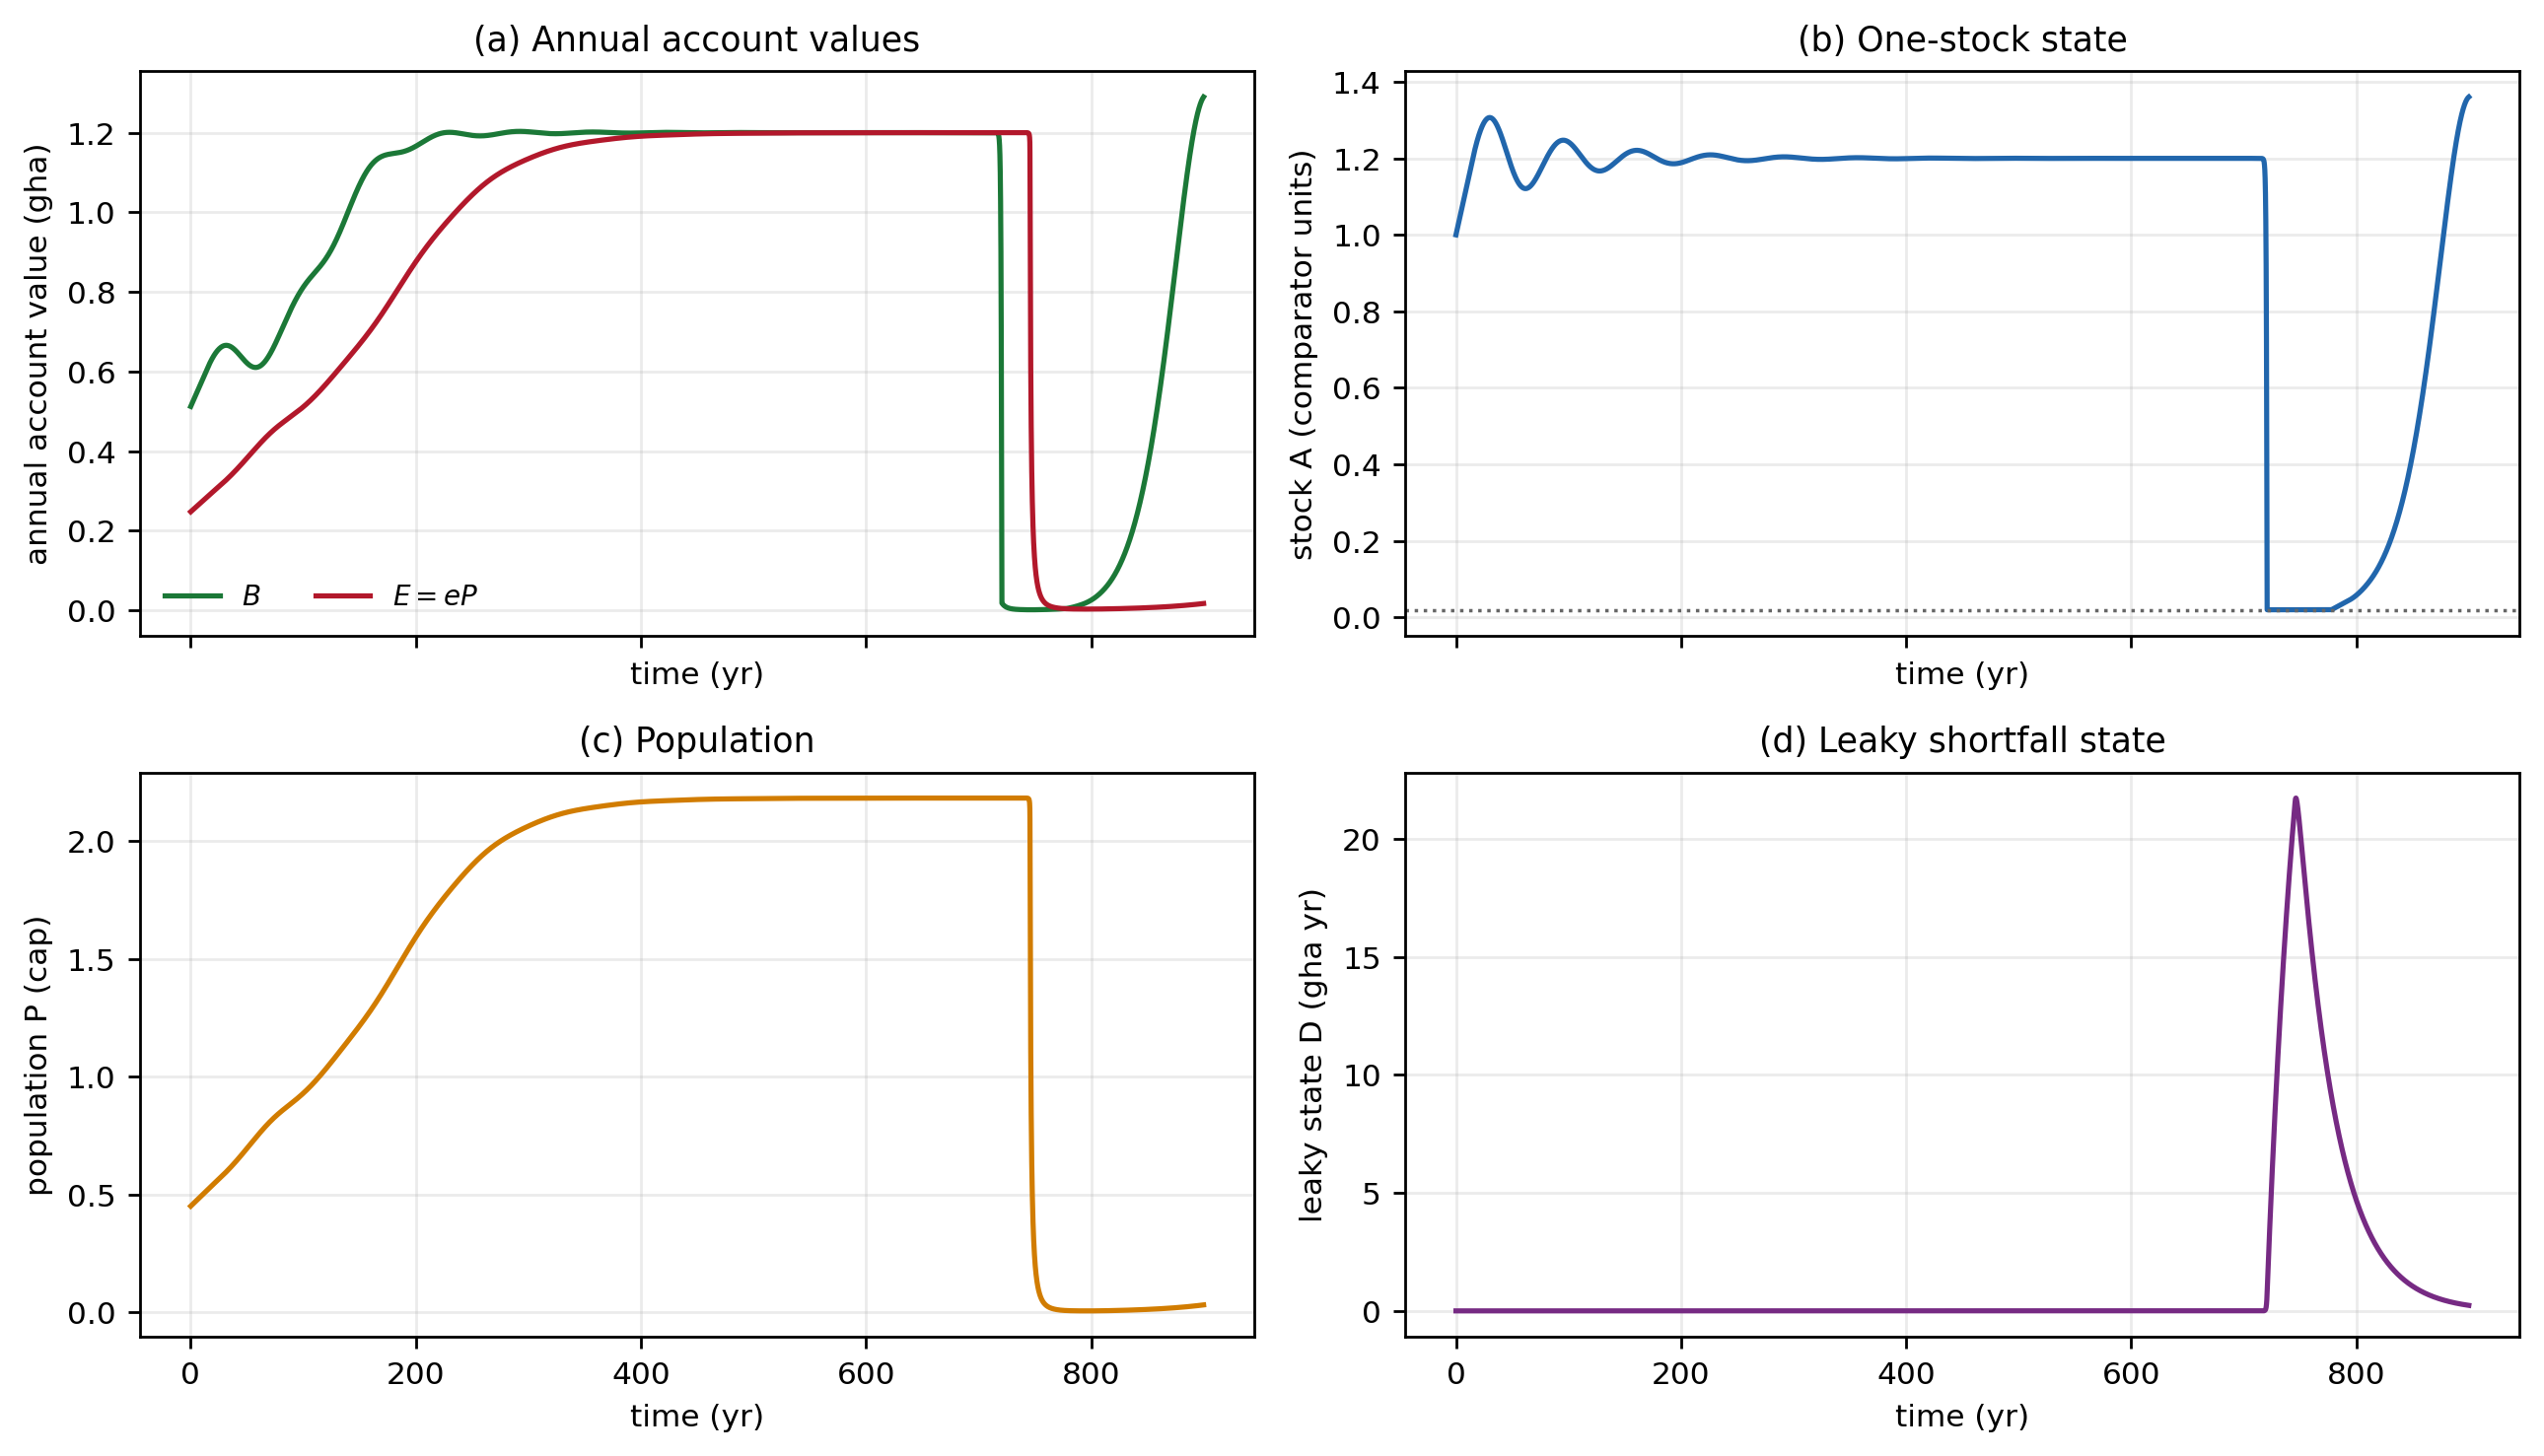
\includegraphics[width=0.96\textwidth]{si_onestock_full_trajectory}
\caption{Full delayed one-stock comparator with a logistic technology increment. Parameters: $A_0=1.0$ stock unit, $P_0=0.45$\,cap, $b_0=0.5$, $b_G=0.6$, $\rho=0.08$\,yr$^{-1}$, $A_{\max}=1.2$ stock units, $e=0.55$\,gha\,cap$^{-1}$, $r=0.02$\,yr$^{-1}$, $\eta=0.03$\,yr$^{-1}$, $\alpha=0.2$\,gha$^{-1}$\,yr$^{-1}$, $\tau_g=15$\,yr, $\tau_p=25$\,yr, $A_{\mathrm{ext}}=0.02$ stock units, $K_{\min}=10^{-4}$\,cap, $\Delta b=0.5$\,gha per stock unit, $\kappa=0.04$\,yr$^{-1}$, and $t_w=120$\,yr; $\sigma=1$, $\omega_{Tb}=1$, and $D_0=0$. The positive-part operator is exact. $B$ and $E$ are in gha, $A$ in comparator-specific stock units, $P$ in cap, and $D$ in gha\,yr. The trajectory reaches the imposed lower bound near $721$\,yr and subsequently recovers as modeled demand falls; the bound is not absorbing. This is a conditional model illustration, not an observation or a two-land result.}
\label{fig:si_onestock_full}
\end{figure}

\begin{figure}[htbp]
\centering
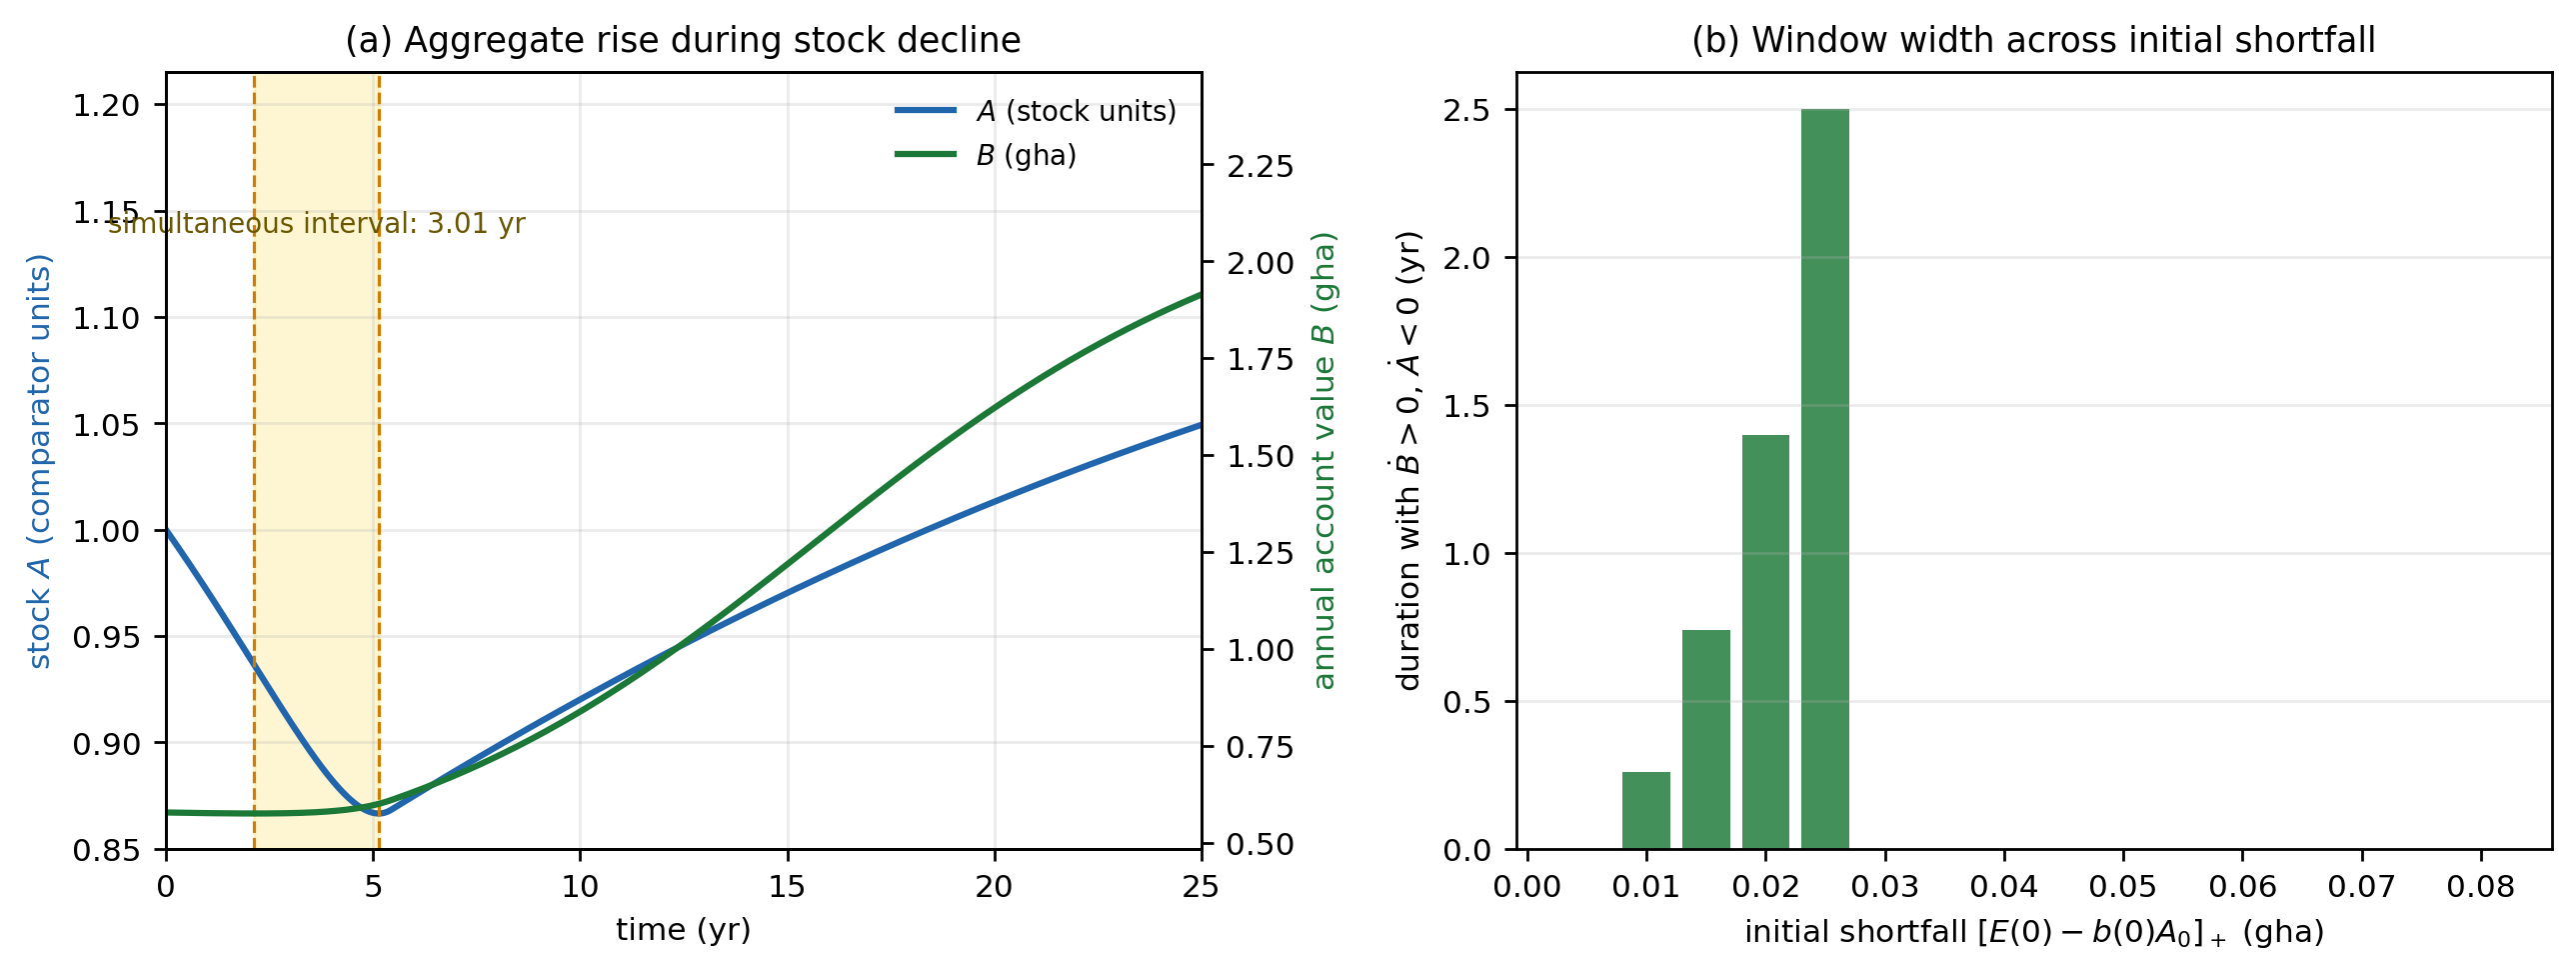
\includegraphics[width=0.96\textwidth]{si_onestock_mask_window}
\caption{One-stock masking example with fixed demand and no delays. Parameters: $A_0=1.0$ stock unit, $E=0.60$\,gha, $b_0=0.5$, $b_G=0.8$, $\rho=0.05$\,yr$^{-1}$, $A_{\max}=1.2$ stock units, $\eta=0.05$\,yr$^{-1}$, $\alpha=0.03$\,gha$^{-1}$\,yr$^{-1}$, $\Delta b=1.5$\,gha per stock unit, $\kappa=0.2$\,yr$^{-1}$, and $t_w=15$\,yr; $\sigma=1$, $\omega_{Tb}=1$, and $D_0=0$. Under the exact positive-part operator, the interval with $\dot B>0$ and $\dot A<0$ lasts about $3.0$\,yr; over it, $A$ falls from about $0.937$ to $0.867$ stock units while $B$ rises from about $0.575$ to $0.600$\,gha. Panel (b) shows the interval width across initial shortfalls $[E(0)-b(0)A_0]_+$ for this parameterization. These are conditional comparator outputs.}
\label{fig:si_onestock_mask}
\end{figure}

\begin{figure}[htbp]
\centering
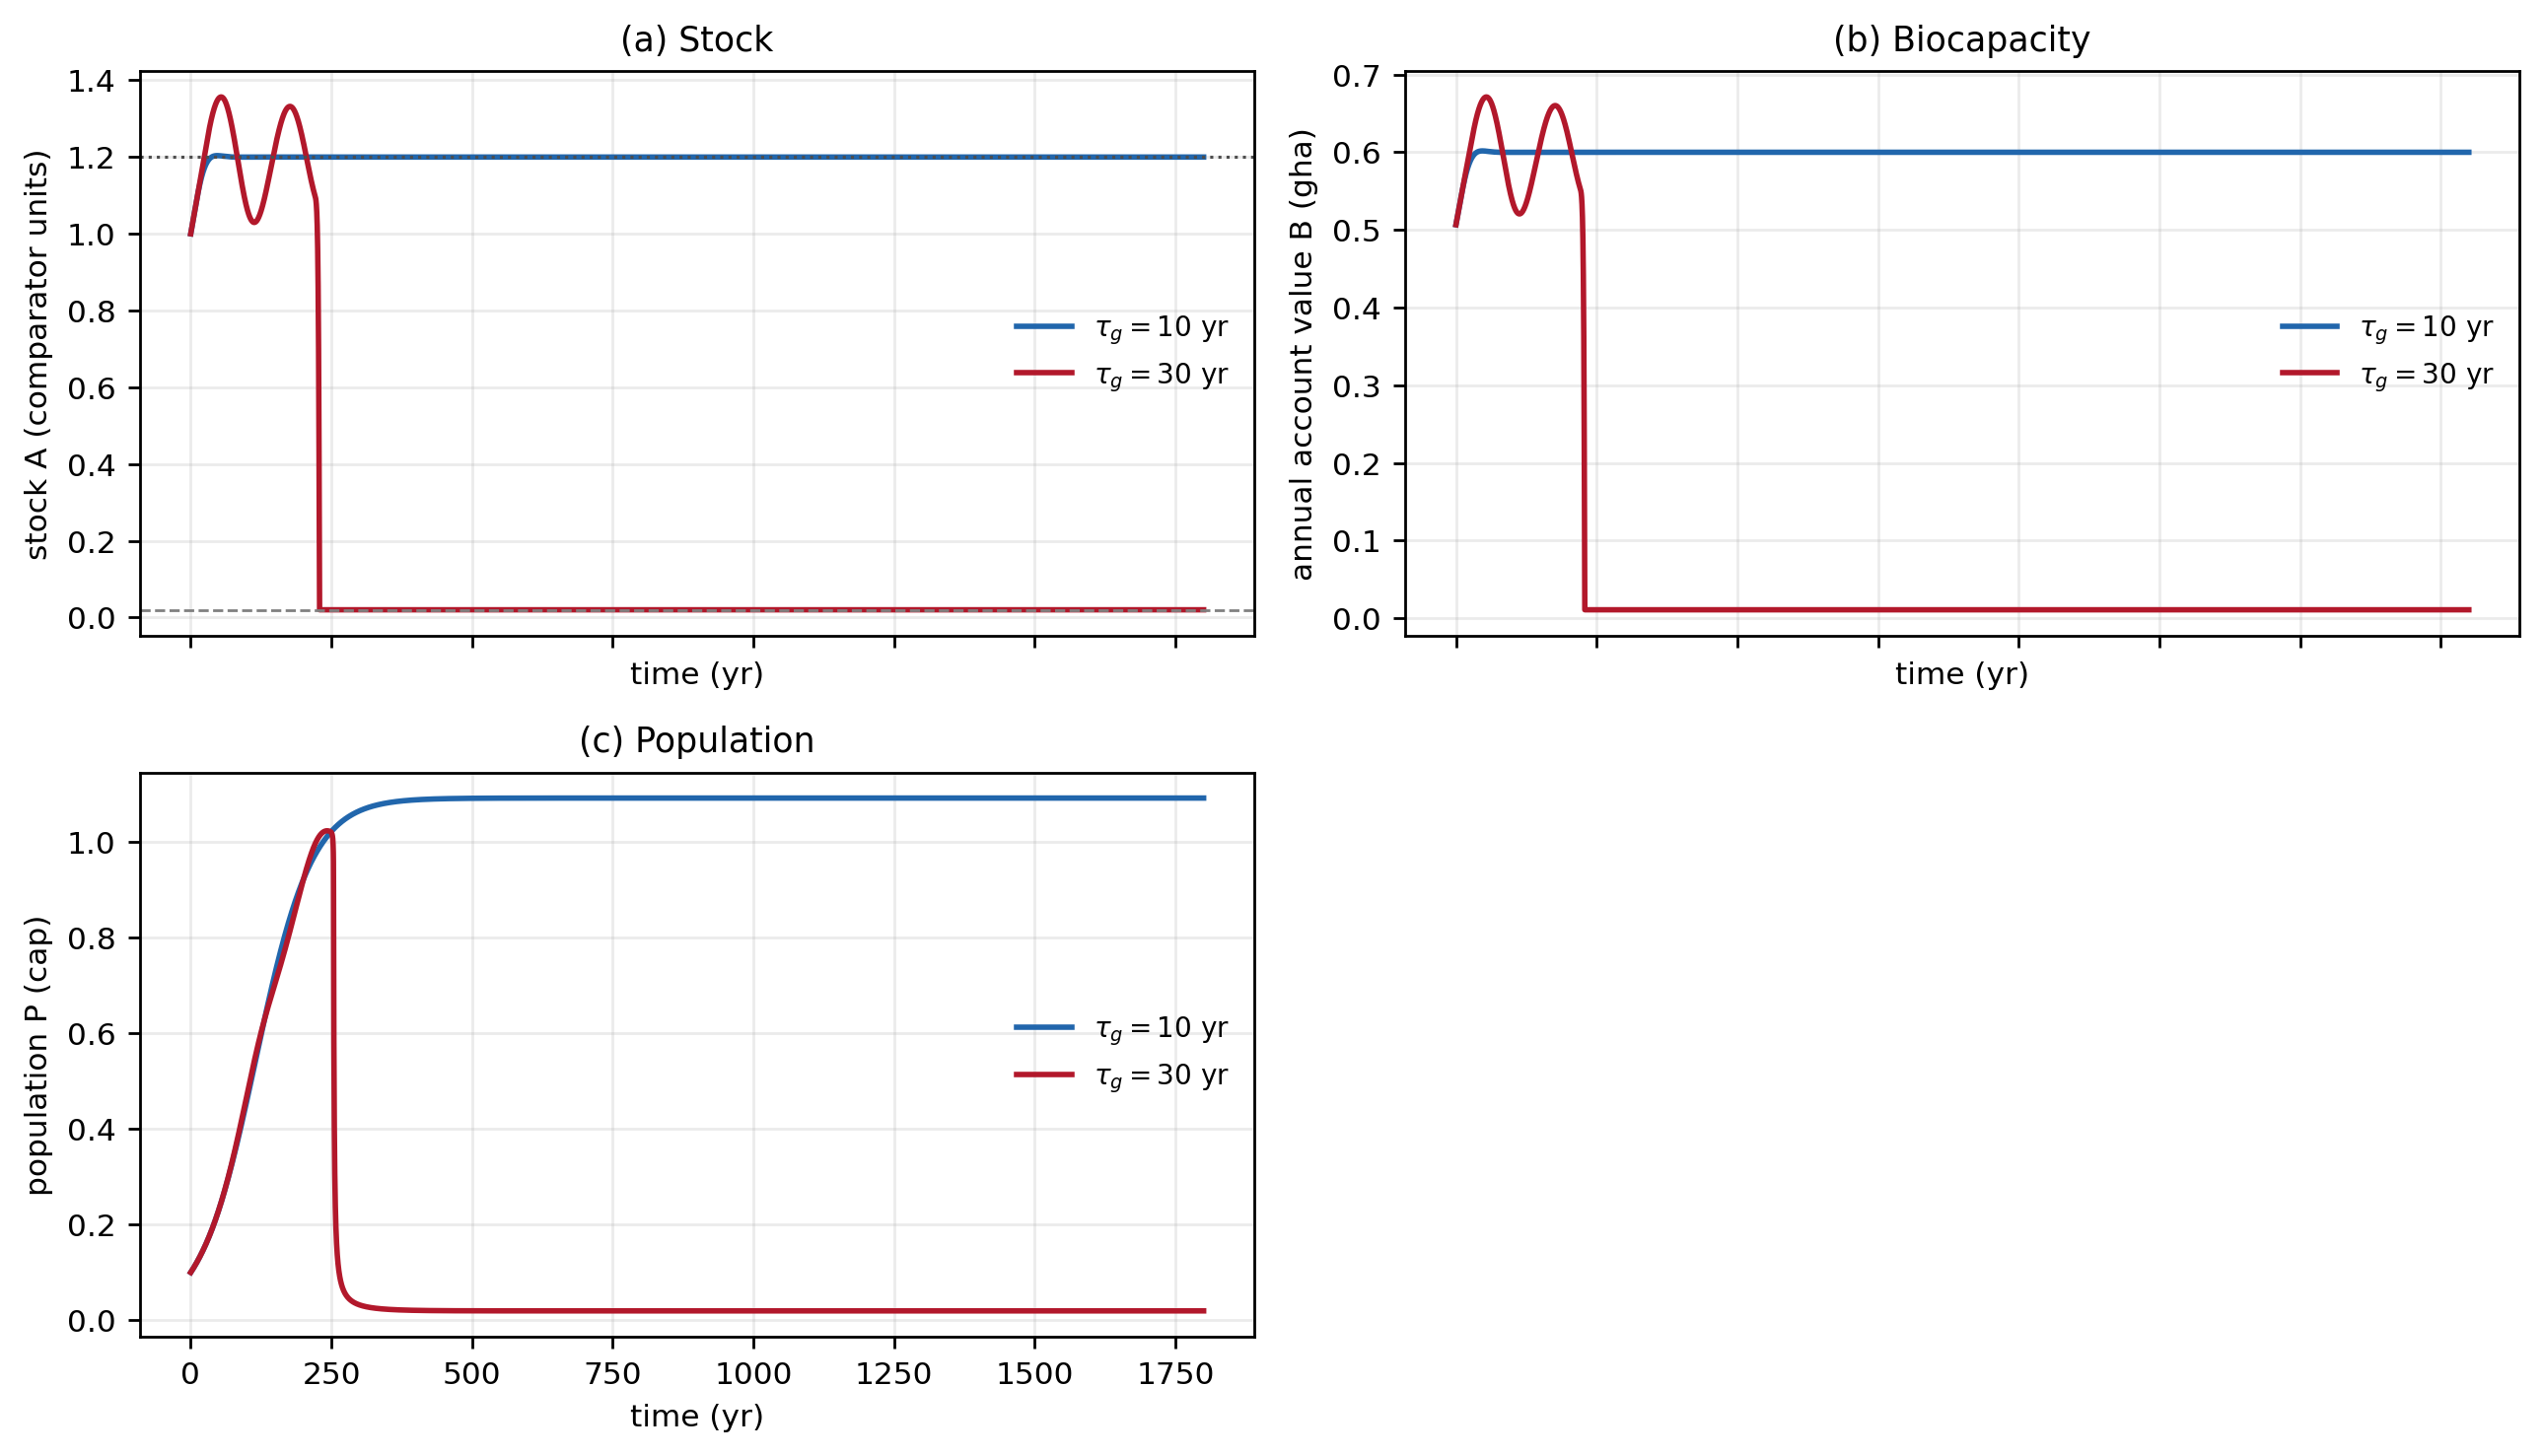
\includegraphics[width=0.96\textwidth]{si_onestock_delay_examples}
\caption{Controlled regeneration-delay examples in the debt-free one-stock subsystem. Both runs use $A_0=1.0$ stock unit, $P_0=0.1$\,cap, $b=0.5$, $b_G=0.8$, $\rho=0.05$\,yr$^{-1}$, $A_{\max}=1.2$ stock units, $e=0.55$\,gha\,cap$^{-1}$, $r=0.02$\,yr$^{-1}$, $\tau_p=25$\,yr, $A_{\mathrm{ext}}=0.02$ stock units, $K_{\min}=10^{-6}$\,cap, and $\sigma=1$; only $\tau_g$ differs ($10$ versus $30$\,yr). $B$ is in gha, $P$ in cap, and $A$ in comparator-specific stock units. The selected trajectories do not determine a general critical delay.}
\label{fig:si_onestock_delay}
\end{figure}

\begin{figure}[htbp]
\centering
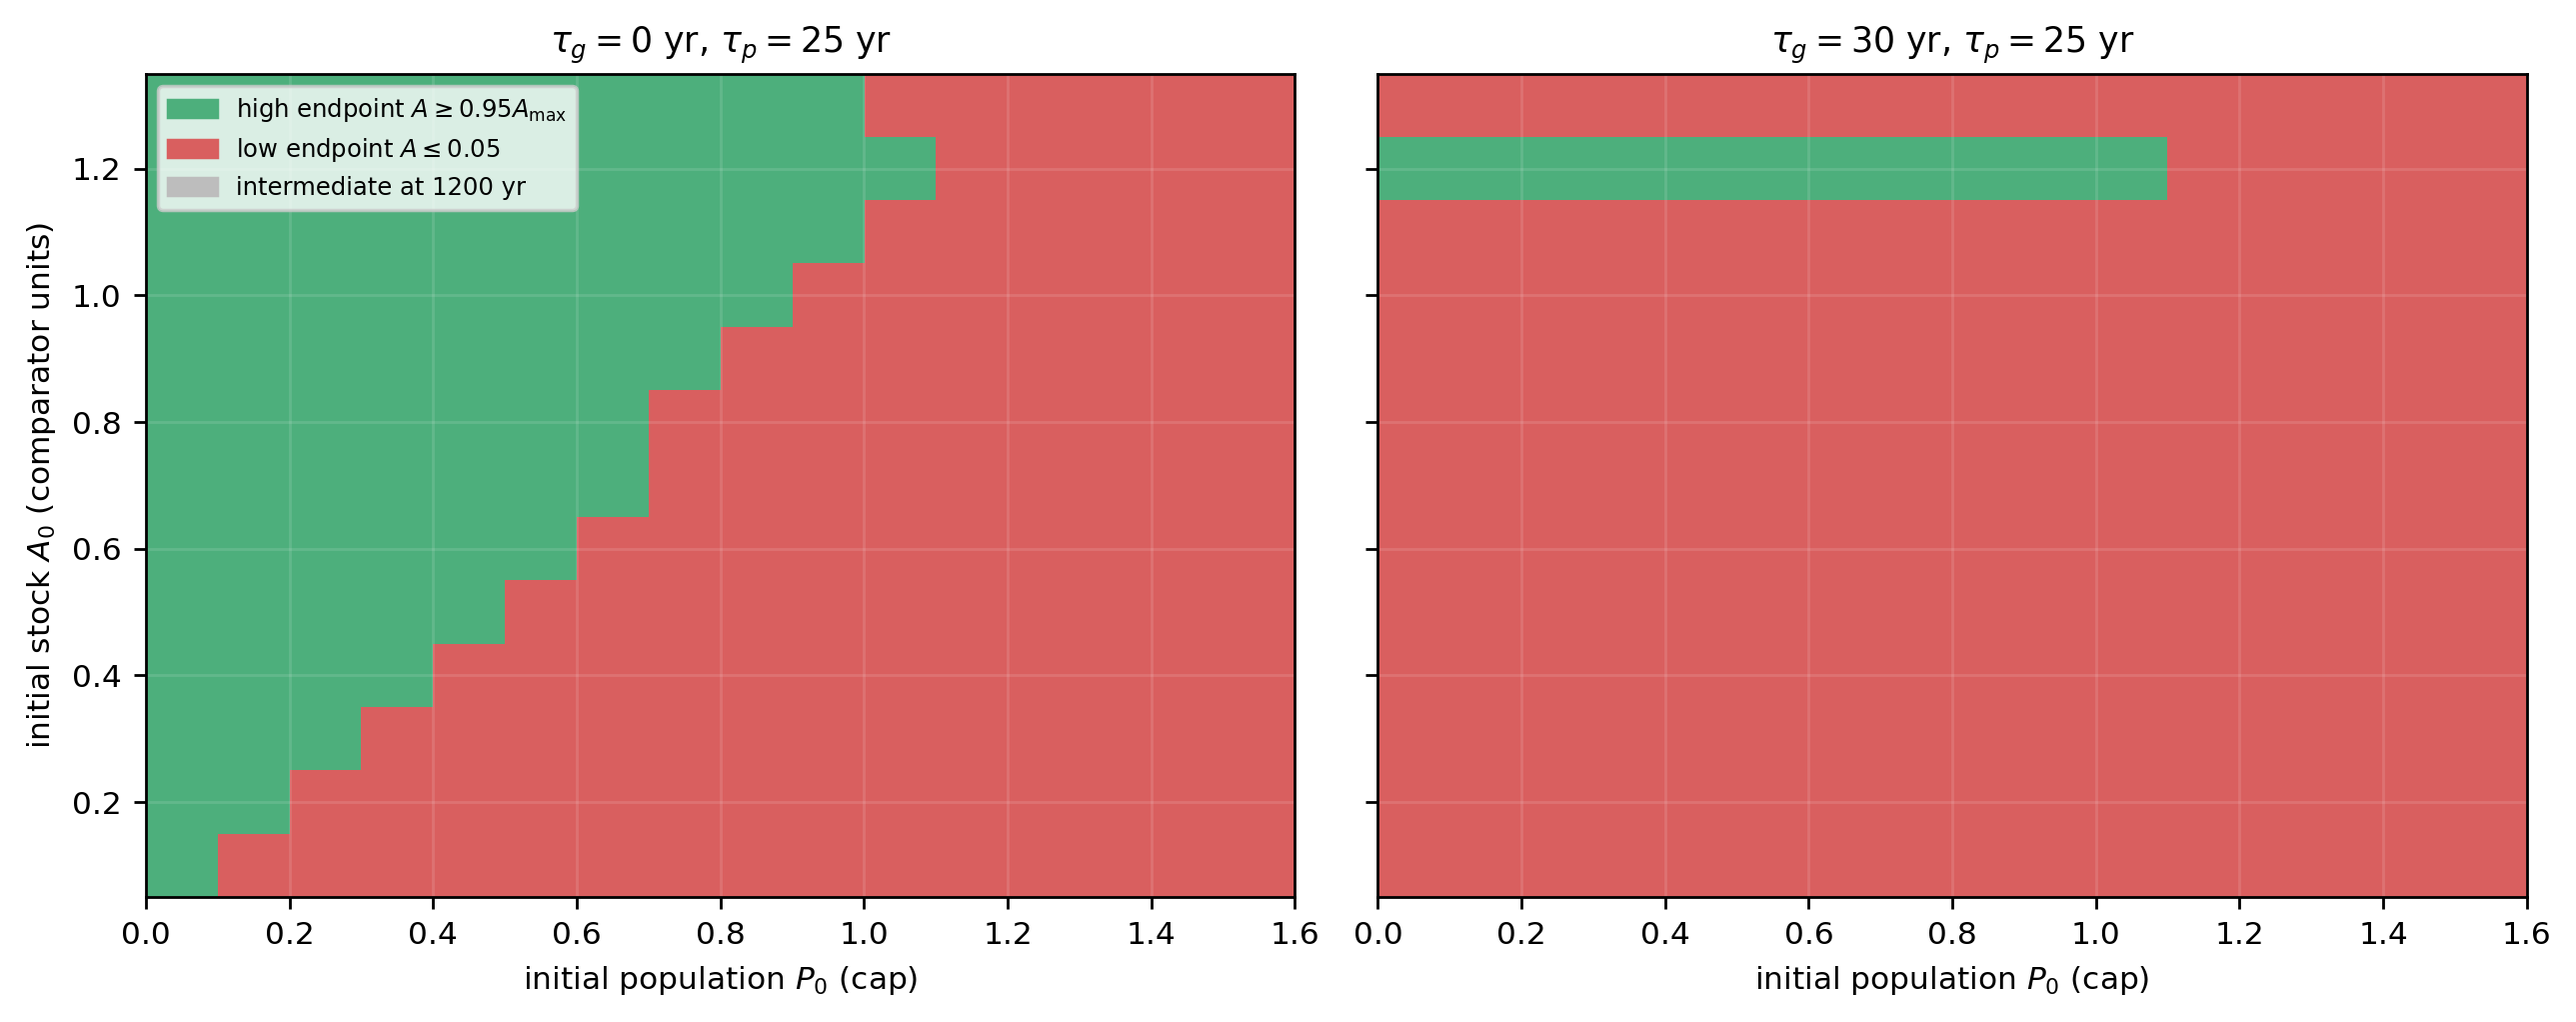
\includegraphics[width=0.96\textwidth]{si_onestock_basin}
\caption{Finite-grid initial-condition classification in the debt-free one-stock subsystem. The debt-free runs use the same parameter set as Fig.~\ref{fig:si_onestock_delay}, with $K_{\min}=10^{-6}$\,cap and $\tau_p=25$\,yr; $\tau_g=0$\,yr in the left panel and $30$\,yr in the right; the imposed lower bound is $A_{\mathrm{ext}}=0.02$ stock units. The grid is $A_0=0.10,0.20,\ldots,1.30$ stock units and $P_0=0.05,0.15,\ldots,1.55$\,cap; trajectories are integrated to $1200$\,yr with $\Delta t=0.5$\,yr. Green denotes a high endpoint $A(1200)\ge0.95A_{\max}$, red a low endpoint $A(1200)\le0.05$ stock units, and gray an intermediate endpoint. These display-grid classifications are not probabilities or continuous-basin measures.}
\label{fig:si_onestock_basin}
\end{figure}

\section{Controlled technology-wave experiment}\label{si:tbwave}

The matched experiment compares endogenous-demand runs with $T_b$ active or inactive, using $P_0=1.0$ or $1.2$\,cap. Both runs in each pair share $A_{tot}=2.5$\,ha, $A_{f0}=0.6$\,ha, $A_{c0}=0.9$\,ha, $q_0=0.9$, and $D_0=0.0$\,gha\,yr. Parameter values and numerical methods match; only $\omega_{Tb}$ differs. The common pre-run histories are constant at $q_0=0.9$ and the no-wave initial account value $B=0.560184$\,gha in both runs. Shared parameters are $b_{f0}=0.85$\,gha\,ha$^{-1}$, $b_c=0.05$\,gha\,ha$^{-1}$, $b_{G,c}=0.8$\,gha\,yr\,ha$^{-1}$, $\rho_c=0.08$\,yr$^{-1}$, $\alpha=0.03$\,gha$^{-1}$\,yr$^{-1}$, $\eta=0.05$\,yr$^{-1}$, $\eta_f=0.05$\,yr$^{-1}$, $\mu=0.06$\,yr$^{-1}$, $e=0.55$\,gha\,cap$^{-1}$, $r=0.02$\,yr$^{-1}$, $\tau_g=20$\,yr, $\tau_p=25$\,yr, $\tau_{conv}=1$\,yr, and $\chi_r=0.10$\,gha$^{-1}$\,yr$^{-1}$. The active-wave parameters are $\Delta b=1.0$\,gha\,ha$^{-1}$, $\kappa_w=0.1$\,yr$^{-1}$, and $t_{wave}=40$\,yr; the integration horizon is $250$\,yr. The logistic increment is nonzero at $t=0$ ($T_b(0)=0.017986$\,gha\,ha$^{-1}$), giving $B(0)=0.560184$\,gha without the wave and $0.570976$\,gha with it. The difference at $t=0$ arises from the logistic tail; the land, quality, population, and debt states are otherwise matched, and the pre-run $B$ history remains common. The wave reaches half its increment at $t_{wave}=40$\,yr.

Figure~\ref{fig:si_wave_debt} shows the $P_0=1.0$ pair. Its all-time debt maximum occurs after the wave midpoint in both runs: $D_{max}=0.008126$\,gha\,yr at $86.15$\,yr without the wave, versus $0.020205$\,gha\,yr at $115.60$\,yr with it. At $P_0=1.2$, by contrast, the all-time maximum occurs early and is lower with the wave, while the maximum over $t\ge t_{wave}$ is higher. Table~\ref{tab:si_wave_debt} reports both all-time maxima and maxima over $t\ge t_{wave}$. Because $t_{wave}$ is the logistic midpoint, the post-midpoint window includes the continued rise of the wave.

\begin{table}[htbp]
\centering\small
\caption{Matched technology-wave/no-wave debt maxima. Entries are $D_{max}$ in gha\,yr, with the time of the maximum in years in parentheses; the ratio is wave/no-wave. ``All'' is the maximum over $0\le t\le250$\,yr; $t\ge40$ is the post-midpoint maximum. The $P_0=1.0$ all-time peaks both occur after the midpoint.}
\label{tab:si_wave_debt}
\begin{tabularx}{\textwidth}{r l r l >{\centering\arraybackslash}X >{\centering\arraybackslash}X r}
\toprule
$P_0$ (cap) & quality update & $\Delta t$ (yr) & window & no wave $D_{max}$ (time) & wave $D_{max}$ (time) & ratio \\
\midrule
$1.0$ & delayed & $0.050$ & all & $0.008126\ (86.15)$ & $0.020205\ (115.60)$ & $2.487$ \\
$1.0$ & delayed & $0.025$ & all & $0.008105\ (86.20)$ & $0.020195\ (115.65)$ & $2.492$ \\
$1.0$ & current & $0.050$ & all & $0.008326\ (85.70)$ & $0.020168\ (115.60)$ & $2.422$ \\
$1.2$ & delayed & $0.050$ & all & $0.061218\ (1.65)$ & $0.051037\ (1.45)$ & $0.834$ \\
$1.2$ & delayed & $0.050$ & $t\ge40$ & $0.010854\ (81.70)$ & $0.025184\ (112.55)$ & $2.320$ \\
$1.2$ & delayed & $0.025$ & all & $0.060732\ (1.625)$ & $0.050582\ (1.475)$ & $0.833$ \\
$1.2$ & delayed & $0.025$ & $t\ge40$ & $0.010808\ (81.775)$ & $0.025165\ (112.625)$ & $2.328$ \\
\bottomrule
\end{tabularx}
\end{table}

For $P_0=1.0$, the all-time wave/no-wave debt-peak ratio is $2.487$ at $\Delta t=0.05$\,yr, $2.492$ at $0.025$\,yr, and $2.422$ under the current-quality specification at $0.05$\,yr. For $P_0=1.2$, the corresponding all-time ratios are $0.834$ and $0.833$, while the post-midpoint ratios are $2.320$ and $2.328$. Debt maxima change by less than $0.9\%$ under step halving. In the $P_0=1.0$ pair, $A_c$ does not fall below its initial value of $0.9$\,ha; the experiment therefore illustrates a conditional delayed debt rebound, not the capital-land drawdown in the frozen-demand baseline. The $P_0=1.2$ contrast shows that the all-time maximum and the post-midpoint maximum are distinct summaries. $D$ is the model's leaky time-integral of shortfall, not an observed NFA or physical-stock variable.

\begin{figure}[!htbp]
\centering
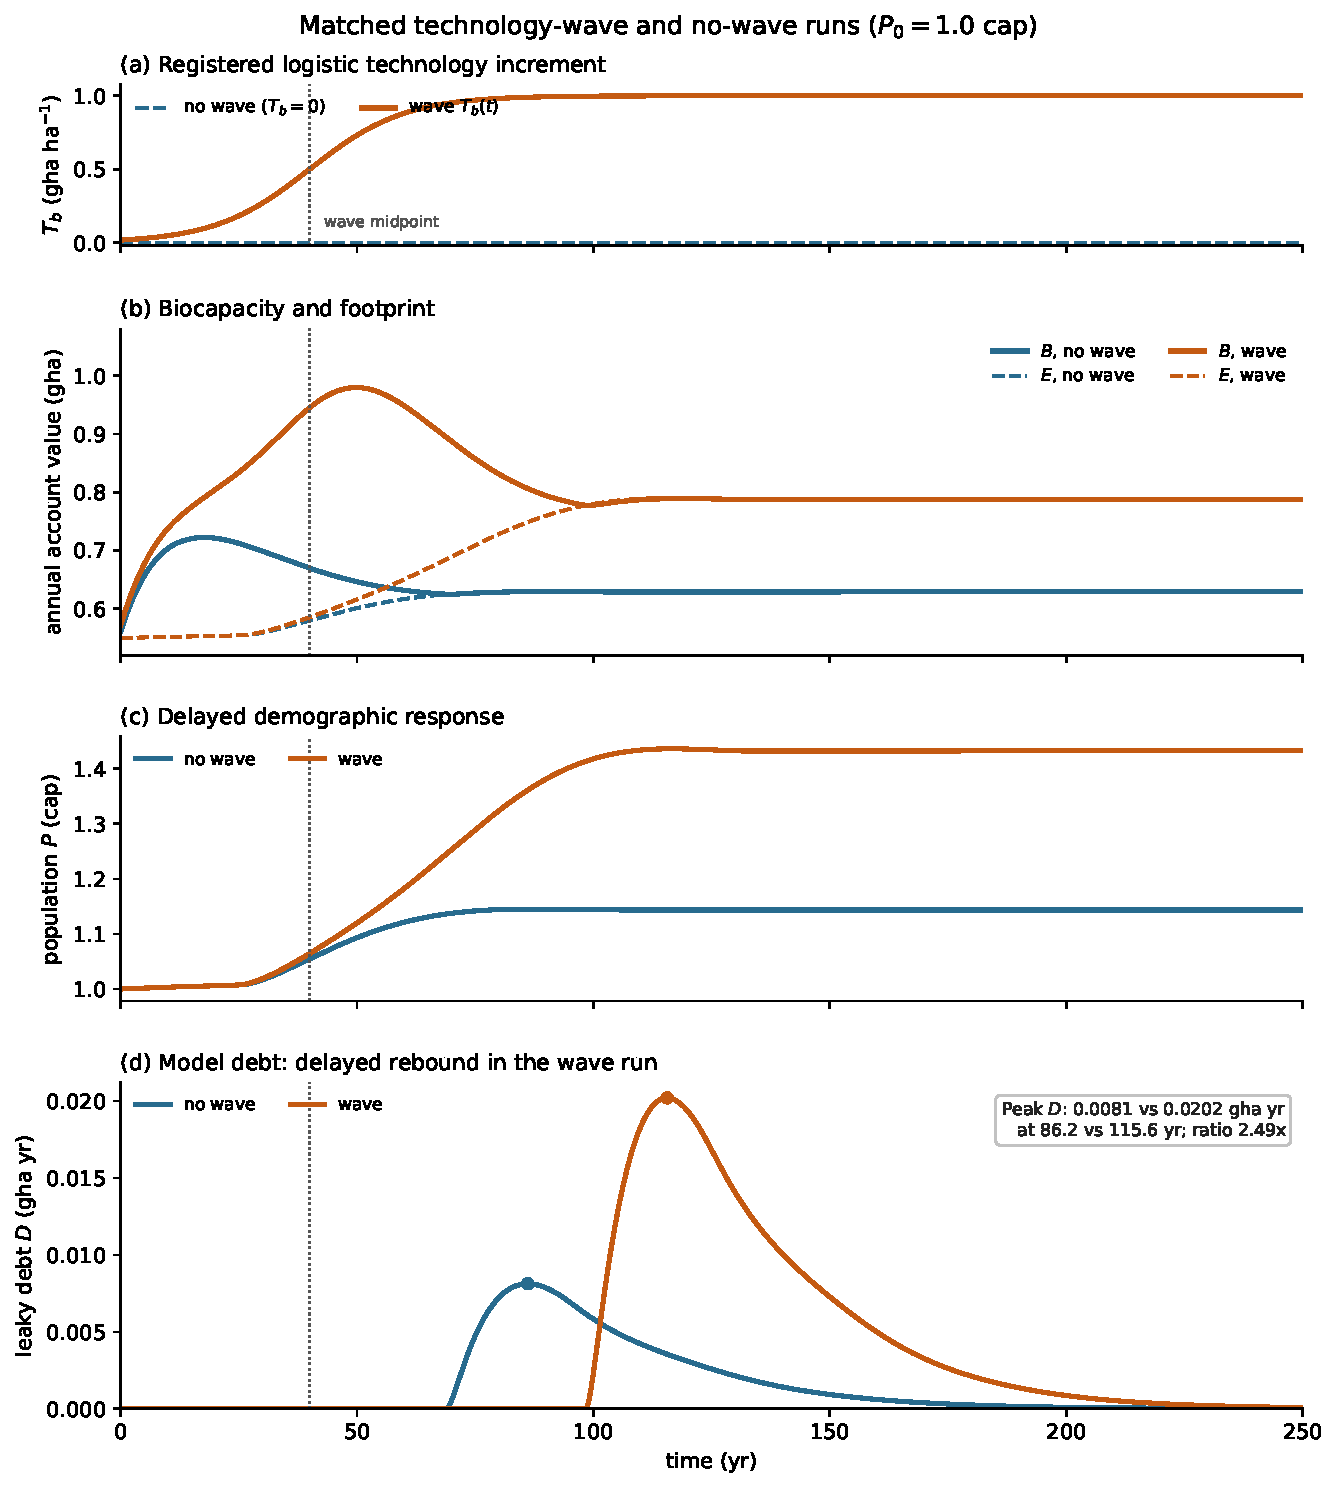
\includegraphics[width=0.92\textwidth]{fig_tb_wave_debt}
\caption{Matched endogenous-demand technology-wave/no-wave simulation at $P_0=1.0$\,cap. Parameters and initial conditions are listed in SI~\S S8; only $T_b$ is switched on or off. (a) The active logistic increment $T_b(t)$, with the dotted line at its midpoint $t_{wave}=40$\,yr; (b) annual account values $B$ and $E$ (gha); (c) population $P$ (cap); (d) leaky model debt $D$ (gha\,yr). Markers denote all-time maxima, which occur at $86.15$\,yr without the wave and $115.60$\,yr with it; peak debt is $0.008126$ versus $0.020205$\,gha\,yr. The plotted wave begins with its small logistic tail at $t=0$ and approaches $\Delta b=1.0$\,gha\,ha$^{-1}$; the dotted line marks the midpoint, not an end date.}
\label{fig:si_wave_debt}
\end{figure}

\section*{Supplementary references}
\begin{thebibliography}{99}
\small
\bibitem[{Abaee(2026b)}]{Abaee2026b} Abaee, A. (2026b). \emph{Aggregation is a claim, not a presentation: the geometry of the acceptance gap between compensatory and noncompensatory transition assessment}. Working paper (v71). \url{https://github.com/MIKEAA2020/general-sustainability/blob/2efaa62083f2007dec3446c15c475af88f0925f3/arena%20agent%201/paper%20rewrites/latex/paper06_assessment_separation_v71.pdf}.
\bibitem[{Abaee(2026a)}]{Abaee2026a} Abaee, A. (2026a). \emph{Governance delay and the stability of harvested stocks: mobilising and protective feedback rules, and the review interval as a design parameter}. Working paper (v41). \url{https://github.com/MIKEAA2020/general-sustainability/blob/2efaa62083f2007dec3446c15c475af88f0925f3/arena%20agent%201/paper%20rewrites/latex/paper4_delay_dynamics_v41.pdf}.
\bibitem[{Global Footprint Network(2009)}]{GFNStandards2009} Global Footprint Network (2009). \emph{Ecological Footprint Standards 2009}. Global Footprint Network. \url{https://www.footprintnetwork.org/content/uploads/2019/05/Ecological_Footprint_Standards_2009.pdf}.
\bibitem[{Global Footprint Network(2019)}]{GFNGuidebook2019} Global Footprint Network (2019). \emph{Working Guidebook to the National Footprint Accounts 2019}. Global Footprint Network. \url{https://www.footprintnetwork.org/content/uploads/2019/05/National_Footprint_Accounts_Guidebook_2019.pdf}.
\bibitem[{Hutchinson(1948)}]{Hutchinson1948} Hutchinson, G. E. (1948). Circular causal systems in ecology. \emph{Annals of the New York Academy of Sciences}, 50(4), 221--246.
\bibitem[{Hutchings and Reynolds(2004)}]{HutchingsReynolds2004} Hutchings, J. A. \& Reynolds, J. D. (2004). Marine fish population collapses: consequences for recovery and extinction risk. \emph{BioScience}, 54(4), 297--309.
\bibitem[{Lo et al.(2026)}]{Lo2026NFA} Lo, K., Basnet, N., Miller, E., Srikanthalingam, B., Foley, B., Van Berkum, J. L., Long, A. H., Toneva, P., Ermina, M. \& Klinkenberg, C. (2026). \emph{National Ecological Footprint and Biocapacity Accounts, Edition 2026 (1961--2025): Results and metadata, version 1.0.} Prepared for Footprint Data Foundation by researchers at York University and the University of Iceland. Workbook: \url{https://footprint.info.yorku.ca/files/2026/04/NEFBA_Data_global_national_ecological_footprint_biocapacity.xlsx}; release notes: \url{https://footprint.info.yorku.ca/files/2026/04/NEFBA_ReleaseNotes.pdf}; data page: \url{https://footprint.info.yorku.ca/data/}.
\bibitem[{Neubauer et al.(2013)}]{Neubauer2013} Neubauer, P., Jensen, O. P., Hutchings, J. A. \& Baum, J. K. (2013). Resilience and recovery of overexploited marine populations. \emph{Science}, 340(6130), 347--349.
\bibitem[{Our~World~in~Data(2026a)}]{OWIDCereal2026} Our~World~in~Data (2026a). \emph{Cereal yield.} FAOSTAT data accessed through Our World in Data; grapher page last updated 25 February 2026; accessed 24 October 2026. \url{https://ourworldindata.org/grapher/cereal-yield}.
\bibitem[{Our~World~in~Data(2026b)}]{OWIDCropland2026} Our~World~in~Data (2026b). \emph{Cropland area.} FAOSTAT data accessed through Our World in Data; grapher page last updated 25 February 2026; accessed 24 October 2026. \url{https://ourworldindata.org/grapher/cropland-area}.
\bibitem[{Poeplau et al.(2011)}]{Poeplau2011} Poeplau, C., et al. (2011). Temporal dynamics of soil organic carbon after land-use change in the temperate zone--carbon response functions as a model approach. \emph{Global Change Biology}, 17(7), 2415--2427.
\bibitem[{Poorter et al.(2016)}]{Poorter2016} Poorter, L., et al. (2016). Biomass resilience of Neotropical secondary forests. \emph{Nature}, 530(7590), 211--214.
\bibitem[{United Nations et al.(2021)}]{UN2021SEEA_EA} United Nations et al. (2021). \emph{System of Environmental-Economic Accounting---Ecosystem Accounting (SEEA EA).} White cover publication, pre-edited text subject to official editing. New York: United Nations. \url{https://seea.un.org/ecosystem-accounting}.
\end{thebibliography}

\end{document}
